
\documentclass[draft,linenumbers]{agujournal}
\draftfalse
\journalname{Journal of Advances in Modeling Earth Systems (JAMES)}
\begin{document}


\title{Implementing plant hydraulics in the Community Land Model}
\authors{Daniel Kennedy\affil{1},
Sean Swenson\affil{2},
Keith Oleson\affil{2},
David Lawrence\affil{2},
Rosie Fisher\affil{2},
Pierre Gentine\affil{1}
}


\affiliation{1}{Columbia}
\affiliation{2}{National Center for Atmospheric Research, Table Mesa Drive, Boulder, Colorado, USA}
\correspondingauthor{Daniel Kennedy}{djk2120@columbia.edu}

\begin{keypoints}
\item A simplified soil-plant-atmosphere continuum model based on hydraulic theory is implemented in the Community Land Model (version 5).
\item Prognostic leaf water potential replaces soil matric potential as the functional basis for water stress, thus reflecting how the leaf water supply (via the xylem network) and evaporative demand act in concert to determine plant water status and thus stomatal conductance and leaf gas exchange. 
\item Prognostic root water potential is used to implement hydraulic root water uptake, replacing the heuristic soil 'wilting' factor .
\end{keypoints}



\begin{abstract}
= enter abstract here =
\end{abstract}

%====================
%  INTRODUCTION
%====================

\section{Introduction}

Trees face emerging climate change risk globally \citep{allen2010,anderegg2013b}.
Understanding vegetation response is a high priority, both for discerning climate impacts and for modeling feedbacks to the carbon and hydrological cycles.
In addition to stress from soil moisture drought, vegetation is susceptible to increasing atmospheric transpiration demand \citep{restaino2016,novick2016b}.
Increases in vapor pressure deficit (VPD) have occurred with warming \citep{ficklin2017,seager2015}, and are associated with impacts on vegetation \citep{williams2013,mcdowell2015}.
Significant uncertainty remains regarding how vegetation will respond to changes in hydroclimate within Earth System Models, feeding back onto the carbon cycle as vegetation mediates carbon uptake \citep{dekauwe2017,friedlingstein2014}.


Plant water stress parameterizations are important in Earth System Models, as they define vegetation regulation of surface fluxes (photosynthesis, transpiration) to water fluctuations.
Vegetation water use strategies also modulate carbon uptake, creating a critical coupling between the Earth System's carbon and hydrological cycles \citep{green2017}.
Drought stress parameterizations (functions which relate simple metric of soil moisture status to leaf gas exchange) are widely used to define the response of stomatal conductance to vegetation water status that is used to attenuate transpiration, photosynthesis, and root water uptake with drying.
The dynamics of water stress in models have broad effects on critical land surface processes \citep{joetzjer2014}.
On diurnal timescales, water stress parameterizations influence the partitioning of latent versus sensible heat with effects on surface temperature \citep{bonan2014}.
On longer timescales vegetation water use strategies regulate the global carbon and water cycles \citep{dekauwe2015}.

Many recent studies have aimed at advancing the representation of water flow through the Soil-Plant-Atmosphere continuum (SPAC) in land models \citep{xu2016,christoffersen2016,sperry2017}.
Explicit modeling of water flow through the SPAC adds complexity, but is consistent with evidence of dynamic regulation of vegetation water use in response to both soil and atmospheric drying \citep{sperry2015}.
Furthermore, via Darcy's Law, SPAC models have a robust physical basis.
SPAC models involve new parameters, which presents new challenges \citep{drake2017}, but plant hydraulic trait information is available \citep{kattge2011,anderegg2015a}, providing guidance on parameter estimation.   and can be informative of forest vulnerability to drought \citep{choat2012}.
Likewise vegetation water status observations are available at a scale that is directly relevant to model development \citep{konings2016,grant2016} and can be used to validate model results \citep{momen2017,konings2017b}.

The empirical representation of vegetation water stress in the Community Land Model (CLM) and other land surface models is a known deficiency, with implications for the representation of the dry/wet season in tropical rainforests \citep{powell2013,ukkola2016}.

In this study, we develop a  plant hydraulic implementation within the recently released CLM version 5 (CLM5), based on hydraulic theory, which we refer to as the 'Plant Hydraulic Stress' (PHS) configuration. We analyse the dynamics of the new PHS model  using site-level simulations that replicate the Caxiuan\~a, Brazil through-fall exclusion experiment \citep{fisher2006}.

Advancing the representation of the SPAC introduces the representation of vegetation water potential (discretized into leaf, stem and root elements) into the CLM, as well as an explicit representation of water supply, from the soil through the vegetation substrate. Transpiration is attenuated with drought stress according to vegetation water status, capturing dynamic vegetation water use regulation. These changes have numerous implications, including 


1. Leaf water potential serves as an improved metric for water status (compared to soil water or soil matric potential), since it reflects vegetation sensitivity to both soil and atmospheric drying, while serving as a diagnostic for excessive xylem tension and cavitation risk. 

2. Modeling  and plant hydrodynamics provides a framework for representing hydraulic redistribution \citep{lee2005} 

3. Modeling vegetation water potential allows improved connection to remote sensing observations (e.g. Vegetation Optical Depth) \citep{konings2016}. 

4. Further, root water potential can be used to predict gradient-based root water uptake based on Darcy's law, replacing the previous empirical transpiration partitioning heuristic.  This provides the means to vary, for example, the mean depth of extraction with changing soil water conditions.

5. The new model can represent a range of water use strategies, improving the connection between plant carbon allocation decisions and water availability.



SAY IN WHICH SECTION WE WILL FINE EACH PART

To assess the new model formulation, we carried out site-level simulations at Caxiuan\~a National Forest in Brazil, which features a critical biome (terra-firme moist tropical evergreen forest).  Starting in 2001, a plot at this site was subjected to an approximately 50\% percent precipitation through-fall exclusion.  Due to the large drop in soil moisture at the precipitation exclusion site, we expect and observe \citep{fisher2007} significant vegetation regulation of transpiration and photosynthesis.

In this paper we 
1. Introduce the PHS theory and implemention in the CLM
2. Analyze the dynamics of modeled water stress, root water uptake and soil moisture profiles. 
3. Compare PHS to the behaviour of the default  CLM water stress configuration.
4. Discuss the benefits and limitations of the new model. 

%====================
%  MODEL DESCRIPTION
%====================
\section{Model Description}

%Photosynthesis
\subsection{Photosynthesis}
\label{sect:A}
    The CLM5 photosynthesis model is described in \citet{bonan2011}, \citet{thornton2007},
    and \citet{oleson2013}.Photosynthesis is defined in three regimes: Rubisco-limited, light-limited, and export-limited 
    following \citet{farquhar1980} and \citet{harley1992}.The implementation extends \citet{sellers1996a,sellers1996b} with 
    co-limitation following \citet{collatz1991}. 
    
    CLM5 photosynthesis, in its default configuration, is a two-big-leaf model, with a sunlit and shaded leaf for each plant functional type \citep{thornton2007, dai2004, oleson2013}. 
    The canopy fluxes module iterates the solution for leaf temperature to satisfy the leaf surface energy balance, while environmental conditions are evolving.
    Within this, the photosynthesis module further iterates to solve for inter-cellular CO$_2$ concentration, balancing stomatal flux of 
    CO$_2$ with photosynthetic assimilation flux of CO$_2$.
    

%Stomatal Conductance
\subsection{Stomatal Conductance}
\label{sect:gs}
    CLM5 implements the Medlyn stomatal conductance model, which reconciles the empirical and optimal approaches to modeling 
    stomatal conductance \citep{medlyn2011}. 
    Stomatal conductance of CO$_2$ is thus directly related to net photosynthesis ($A_n$), CO$_2$ concentration at the leaf surface 
    ($C_a$), and the square root of the vapor pressure deficit near the leaf surface ($\sqrt{D}$).
    \begin{equation}
    g_s=g_0+\left(1+\dfrac{g_1}{\sqrt{D}}\right)\dfrac{A}{C_a}
    \end{equation}
    The model features two parameters $g_0$ ($\mu$mol / m2 / s) and $g_1$ (kPa$^{0.5}$). 
    The $g_0$ parameter is minimum stomatal conductance, representing cuticular and epidermal losses (small). 
    The $g_1$ parameter relates to the marginal water cost guiding the optimization of carbon assimilation. These parameters are plant functional type dependent.
    
    The Medlyn model, derived from stomatal optimization theory, predicts stomatal conductance to maximize assimilation relative to water costs ($A-\lambda E$), 
    but does not resolve concurrent limitations to stomatal conductance associated with drought conditions.   These water stress factors (in our case, $f_w$), are used to represent stomatal and non-stomatal limitation not captured by the leaf-level stomatal conductance model (which can be thought of as a prediction of maximum stomatal conductance in these cases). To represent soil drought, and its impact on diffusive fluxes, land surface models typically include a `water stress factor'($f_w$, dimensionless, 0 to 1, formerly $\beta_t$). Uncertainty remains within the literature for how to apply water stress factors to photosynthesis and/or stomatal conductance. 
    \citep{zhou2013,novick2016a,sperry2015}.
    
    In CLM, $f_w$ multiplies the rate of maximum carboxylation ($V_{\text{cmax}}$) as described in \citet{oleson2013}. Other models opt for soil-moisture based stomatal limitation (linking the stomatal conductance model slope parameter to soil moisture), however,
    \cite{lin2018} found that only $g_0$ was sensitive to soil moisture (and not $g_1$).
    \cite{zhou2013} suggest that changes in assimilation tend to exceed those predicted by modulating $g_1$ with soil moisture, but could be captured by changing $V_{\text{cmax}}$.
    Other field studies, however, suggest that $V_{\text{cmax}}$ does not change with drought, whereby modeled $V_{\text{cmax}}$ instead may implicitly account for mesophyll conductance changes \citep{flexas2004}.
    
    In PHS, we opt for a simplified form of this stress approach, which seems to be consistent with field observations \citep{lin2018}. Prognostic water stress ($f_w$, ranging from 0-1) attenuates stomatal conductance indirectly via multiplication of $V_{\text{cmax}}$. Water stress then lowers assimilation, which is coupled to stomatal conductance ( \citep{medlyn2011}).
    
    $f_w$ is modeled here as a function of leaf water potential ($\psi_{leaf}$) (see Section \ref{sect:demand}), with stress increasing as $\psi_{leaf}$ becomes more negative.
    This reflects the concept of hydraulic safety, with vegetation avoiding excessive xylem tension associated with risk of cavitation.
    
    Utilizing leaf water potential adopts a framework where stomatal conductance optimized for carbon gain is concurrently limited by hydraulic constraints \citep{novick2016a}. As a result, low soil water (bottom-up stress) can induce leaf moisture stress due to limited water supply while high atmospheric VPD can also induce leaf moisture stress by propagating a drying into the xylem (top-down stress).
    
    
     Much recent work has focused on alternative constraints on plant hydrodynamics, especially in response to drying soils \citep{manzoni2013b,novick2016a,zhou2014}.
    This includes how plants manage the risk of cavitation associated with increasing xylem tension \citep{sperry1998}.
    \citep{sperry2017}, for example, argue that theory based on hydraulic costs (define) could be used instead of optimizing of $A-\lambda E$.  
    Otherwise, the marginal water cost might be adjusted based on  soil water status  by adjusting $\lambda$ or Medlyn $g_1$ \citep{manzoni2013b}, but this may underestimate drought effects on photosynthesis *expand on this-RF*\citep{zhou2013,lin2018}.
    A hybrid approach, combines stomatal optimization with hydraulic constraints and/or
    so-called non-stomatal limitation, where stress attenuates $V_{\text{cmax}}$ or mesophyll conductance (both of which feed back through photosynthesis to lower stomatal conductance) \citep{egea2011,novick2016a}. [*link this back to which options are used in PHS -RF*]

    
% Plant Hydaulics
\subsection{Plant Hydraulic Stress (PHS)}
  The PHS model within CLM5 uses hydraulic (Darcy's) law and a corresponding electrical circuit analogy (Figure \ref{circuit}), to model the flow of water through the SPAC. The hydraulic framework is used to diagnose water stress associated with increasing xylem tension
  and to calculate the root water uptake in each of (in this case) 20 vertically discretized soil layers.

  \begin{figure}[h]
     \centering
     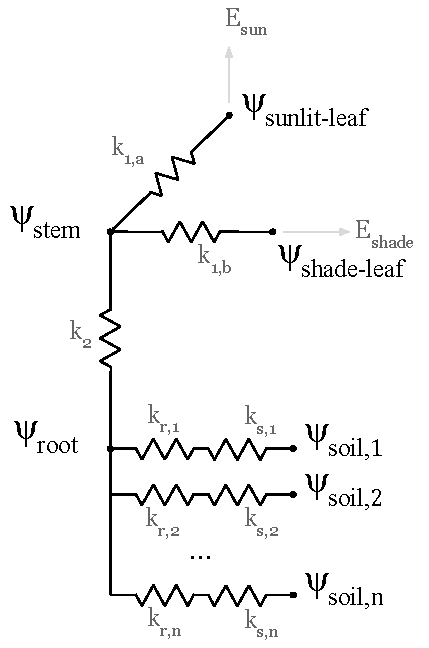
\includegraphics[width=9pc]{../figs/circuit.pdf}
     \caption{Plant hydraulic circuit analog schematic}
     \label{circuit}
  \end{figure}

%Hydraulic schematic and segmentation
  \subsubsection{Hydraulic schematic and segmentation}
  PHS solves for the set of SPAC vegetation water potential values ($\psi_{\text{root}}$, $\psi_{\text{stem}}$, $\psi_{\text{shade-leaf}}$, $\psi_{\text{sun-leaf}}$ ) that matches water supply (root water uptake) to water demand (transpiration), while maintaining continuity of water flow throughout the SPAC. Segmentation and other model design decisions followed a preference for a simplified implementation that whenever possible conformed to existing CLM model structure.
  
  At each node in the circuit diagram in Figure \ref{circuit} we model water potential, and, between nodes, we resolve the flux of water. The choice of nodes for segmentation is designed to take advantage of field-measured hydraulic traits and to allow for differences in segment parameterizations \citep{simonin2015, sperry2015}. As in other versions of the CLM,  PHS uses vertically discretized soil layers and a two-layer (sunlit vs. shaded) canopy.  Water uptake from the different soil layers is assumed to operate in parallel;  a typical assumption justified by higher resistance in lateral versus central roots (e.g. Williams et al. 2001). We further separate resistance through the soil matrix from the resistance through the root tissue \citep{williams1996}. 
  Specifics on the parameterization of conductance for each segment are provided in Appendix B.1.

%Water Supply
    \subsubsection{Water supply}
    \label{sect:supply}
    Water supply is modeled via Darcy's Law, where flow of water ($q$) is the product of the path hydraulic conductance ($k$) and the gradient in water potential (accounting for changes in gravitational potential).  Equation \ref{eq:darcy} represents the flow from a generic node 1 to node 2. 
    
     \begin{linenomath*}
     \begin{equation}
     \label{eq:darcy}
     q = -k\left(\psi_2 - \psi_1 - \rho g \Delta z\right)
     \end{equation}
     \end{linenomath*}
    
    PHS does not represent plant tissue water storage (or capacitance, using the electrical circuit analogy).  Capacitance significantly complicates the water potential solution \citep{celia1990} and is challenging to parameterize \citep{bartlett2016}. However, buffering of water stress provided by tissue water storage could potentially be important especially on sub-daily timescales \citep{meinzer2009,epila2017}, whereby its inclusion may be warranted in future model generations.

     Vegetation segment conductance is modeled following empirical xylem vulnerability curves \citep{tyree1989}, where segments lose conductance with increasing xylem tension related to cavitation and embolism \citep{holbrook2001}. The vulnerability curves model loss of conductance relative to maximum conductance using two parameters: $c_k$, a sigmoidal shape-fitting parameter, and $p_{50}$, the water potential at 50\% loss of segment conductance (following \cite{gentine2016}). 
     
     Both $c_k$ and  $p_{50}$ can be estimated from field experiments \citep{sack2002},  and $p_{50}$ is available in the TRY trait database \citep{kattge2011}. Parameterization based on $p_{50}$ aligns with the call for a transition to models that use a wider range of plant functional trait data in their parameterization \citep{anderegg2015a}. The loss of xylem conductivity is based on lower terminal water potential ($\psi_1$) as is typical in other simplified models \citep{xu2016}, but 
     may underestimate the integrated loss of conductivity \citep{sperry2015}. 
         
     \begin{linenomath*}
     \begin{equation}
     \label{eq:vulnerability}
     k = k_{\text{max}} \, 2^{-\left(\dfrac{\psi_1}{p_{50}}\right)^{c_k}}
     \end{equation}
     \end{linenomath*}
     
     PHS models root, stem, and leaf tissue conductances according to equation \ref{eq:vulnerability}. The parameterization of $k_{\text{max}}$ varies by hydraulic segment (see details in Appendix B1). The conductance across the soil matrix to the root surface follows \citet{williams2001} and \citet{bonan2014} and estimates a characteristic distance between the bulk soil and the root surface, to facilitate length-scaling of soil conductivity. Bulk soil resistivity is based on \citet{clapp1978} as described in \citet{oleson2013}. Further details are provided in Appendix B1.
    
%Water demand
    \subsubsection{Water demand}
    \label{sect:demand}
    
    Vegetation water demand and stomatal regulation is based on the Medlyn stomatal conductance model (see Section \ref{sect:gs}), which we adjust using the water stress factor $f_w$. 
    As discussed earlier, $f_w$ is based on leaf water potential \citep{klein2014}, and multiplies $V_{\text{cmax}}$, thus attenuating photosynthesis, and thus also stomatal conductance and transpiration.
    
     As leaf water potential declines (because of transpiration) and xylem tension increases, transpiration is attenuated relative to its maximal value.  The maximum transpiration ($E_{\text{sun,max}}$, $E_{\text{shade,max}}$) is defined as the value that results from Medlyn stomatal conductance in the absence of water stress (achieved by setting $f_w=1$). The fraction of maximum transpiration is modeled with a two-parameter sigmoidal function (Equation \ref{eq:demand}). 
     
    
     \begin{linenomath*}
     \begin{eqnarray}
     \begin{aligned}
     \label{eq:demand}
     E_{\text{sun}}     &= E_{\text{sun,max}} \, 2^{-\left(\dfrac{\psi_{\text{sun-leaf}}}{\psi_{50}}\right)^{c_k}} \\
     E_{\text{shade}} &= E_{\text{shade,max}} \, 2^{-\left(\dfrac{\psi_{\text{shade-leaf}}}{\psi_{50}}\right)^{c_k}}
     \end{aligned}
     \end{eqnarray}
     \end{linenomath*}
    
     Where $\psi_{50}$, is the leaf water potential at 50\% loss of transpiration and $c_k$ is a sigmoidal shape-fitting parameter.

    
    We define $f_w$ as the ratio of attenuated to maximal stomatal conductance (Equation \ref{eq:stress}).  Maximum stomatal conductance ($g_{\text{s,sun,max}}$, $g_{\text{s,shade,max}}$) is computed as the stomatal conductance in the absence of water stress, i.e. $f_w=1$.  The attenuated stomatal conductance ($g_{\text{s,sun}}$, $g_{\text{s,shade}}$) is then the stomatal conductance associated with the PHS module water flow solution, which matches vegetation water supply with vegetation water demand 
    (Section \ref{sect:solution}).
    
     \begin{linenomath*}
     \begin{eqnarray}
     \begin{aligned}
     \label{eq:stress}
     f_{\text{w,sun}}         &= \dfrac{g_{\text{s,sun}}}{g_{\text{s,sun,max}}} \\
     f_{\text{w,shade}}     &= \dfrac{g_{\text{s,shade}}}{g_{\text{s,shade,max}}} \\
     \end{aligned}
     \end{eqnarray}
     \end{linenomath*}
    
     Whereas the water supply parameters (see Section \ref{sect:supply}) relate to hydraulic traits often measured in the field, the hydraulic demand parameters $\psi_{50}$ and $c_k$ reflect the emergent property of hydraulic limitations to transpiration and must be empirically derived (WHAT ABOUT PLC CURVES?).
     
     CLM also features two empirical stomatal control parameters, which are the soil matric potentials where stomata are either fully closed ($\theta_{wilt}$) or fully open  ($\theta_{crit}$)  (see Section \ref{sect:btran}). Recent modeling studies have proposed different forms of relationship between stomatal regulation with water stress \citep{sperry2017,xu2016,christoffersen2016} and thus this representation remains the topic of active research . 

%PHS solution
    \subsubsection{PHS solution}
    \label{sect:solution}
    
    PHS solves for the set of vegetation water potential values ($\psi$) that matches water supply (root water uptake) to water demand (transpiration), while satisfying continuity across the four water flow segments (soil-to-root, root-to-stem, stem-to-leaf, and leaves-to-transpiration). At each time step, PHS computes the flux divergence $f$ (representing the mismatch of flow in and out of each segment for a given set of vegetation water potential values $\psi_i$, and iteratively updates $\psi$ until convergence is reached in terms of divergence, $f\to0$.
    
    \begin{linenomath*}
    \begin{equation} 
    \psi = \left[
    \begin{array}{c}
    \psi_{\text{sun}} \\ 
    \psi_{\text{shade}} \\ 
    \psi_{\text{stem}} \\ 
    \psi_{\text{root}}            
    \end{array} \right]
    \end{equation}
    \end{linenomath*}
    
    \begin{linenomath*}
    \begin{equation}
    f\left(\psi\right) = \left[ 
    \begin{array}{c}
    E_{sun}-q_{sun}\\
    E_{shade}-q_{shade}\\
    q_{sun}+q_{shade}-q_{stem}\\
    q_{stem}-\sum_{j=1}^n{q_{root,j}}
    \end{array} \right]
    \end{equation}
    \end{linenomath*}
    
    \begin{linenomath*}
    \begin{equation}
    A = \dfrac{df}{d\psi}
    \end{equation}
    \end{linenomath*}    
    
    While $\left|f\right|>0$
    \begin{linenomath*}
    \begin{equation} \begin{aligned}
    \label{eq:iter}
    \Delta\psi &=A^{-1}f\left(\psi_i\right) \\
    \psi_{i+1}  &= \psi_i + \Delta\psi
    \end{aligned} \end{equation}
    \end{linenomath*}    
    
    The numerics are tractable because $f$ has analytical derivatives and $A$ (a 4x4 matrix with six null entries) is easy to invert when well-conditioned. Supply and demand converge, because transpiration demand decreases with more negative leaf water potentials and supply increases with more negative leaf water potentials. Within a set of PHS iterations (\ref{eq:iter}), transpiration is assumed to be linear with $f_w$.
    
    The PHS loop is nested within iterations for intercellular CO$_2$ concentration and leaf temperature. The non-linear relationship between $f_w$ and transpiration is resolved through iteration for converging $f_w$ alongside intercellular CO$_2$. Details on the numerical implementation are provided in Appendix Section B.1.

%====================
%  BTRAN
%====================

\section{Water stress factor, SMS vs. PHS}
\label{sect:btran}
    PHS alters the transpiration beta function ($\beta_t$, colloquially BTRAN ,Equation \ref{bt:1}), SAY WAHT IT IS which is the phenomenological soil water stress function in used in prior versions of CLM, as described in \citet{oleson2013}. Because the name $\beta_t$ is associated with this specific plant hydrodynamics representation, we opt to rename the variable to the water stress factor $f_w$. Throughout this paper we refer to the original CLM plant hydrodynamics framework as SMS (soil moisture stress), as compared to the newer implementation described here, PHS (plant hydraulic stress). We adopt this terminology (in lieu of CLM4.5 vs. CLM5), because SMS is still deployable with CLM5.   In this section we present the SMS version of $f_w$ and outline the differences as compared to PHS
    
    With PHS, we interpret $f_w$ as a drought safety mechanism, attenuating stomatal conductance to avoid excessive xylem tension associated with very negative leaf water potential. As such, $f_w$ is parameterized as a function of prognostic leaf water potential. With SMS, $f_w$ is calculated based on soil matric potential, as a root-fraction weighted average potential departure from an empirical soil layer wilting factor (Equation \ref{bt:1}). Recent studies suggest that the SMS parameterization introduces model bias in turbulent fluxes \citep{bonan2014} and contributes to unrealistic drought response of photosynthesis and stomatal conductance \citep{powell2013}.
    
    In SMS, the variable $f_w$ is unitless, ranging from 0 to 1, with 1 corresponding to no water stress, and 0 corresponding to fully water stressed. It is calculated based on a root-fraction weighted average of soil layer wilting factor ($w_i$), which is a bounded linear function of soil water potential ($\psi_i$) relative to PFT parameters defining the soil potential with stomates fully open ($\psi_{o}$) and fully closed ($\psi_{c}$), among the soil layers $i=1,...\,,n$. Note that root fraction ($r_i$) sums to 1, by definition.
    
    \begin{linenomath*}
    \begin{equation} f_w = \sum_{i=1}^{n}{r_iw_i}
    \label{bt:1}
    \end{equation}
    \begin{equation} 
    \label{bt:2}
    w_i=0 \leq \dfrac{\psi_i-\psi_{c}}{\psi_{o}-\psi_{c}} \leq 1
    \end{equation}
    \end{linenomath*}
    

\subsection{Root water uptake in SMS vs. PHS}
    Such parameterizations (WHICH ONES?) have primarily been examined with application to stomatal conductance, but they are also used to define vegetation soil water extraction. Each timestep, the transpiration flux solution must be distributed among the vertically discretized soil layers. In the SMS framework, the transpiration sink is partitioned by layer according to the soil layer wilting factor and root fraction. 
    
    In both stress parameterizations, $f_w$ multiplies $V_{\text{cmax}}$ to attenuate photosynthesis and stomatal conductance with soil water stress. With SMS, it is also directly used for modeling vegetation water extraction from the soil column. The total transpiration ($T$) is partitioned among the soil layers based on the $f_w$ wilting factor. Within each soil layer, the contribution to total transpiration ($q_i$) depends on the layer root fraction and wilting factor, normalized by $f_w$:

    \begin{linenomath*}
    \begin{equation}
    \label{bt:4}
    q_i = \dfrac{r_i w_i}{f_w}T
    \end{equation}
    \end{linenomath*}
    
    Contrary to the heuristic SMS parameterization, the PHS implementation adopts a physically-based hydraulic framework, where the root water uptake ($q_i$) is the product of the hydraulic conductance ($k_i$) and the gradient in water potential (-$\Delta\psi$) driving the flow, i.e. obeying Darcy's law. That gradient is the difference between the root water potential ($\psi_{\text{root}}$) and the layer soil water potential ($\psi_i$), minus changes in gravitational potential, following Darcy's law.
    
    \begin{linenomath*}
    \begin{equation}
        \begin{aligned}
    q_i &= -k_i \Delta\psi \\
    \Delta\psi &= \left(\psi_{\text{root}}-\psi_{i}-\rho g \Delta z\right)
    \label{phs:sink}
    \end{aligned}
    \end{equation}
    \end{linenomath*}
    
    For comparison between SMS and PHS, we recast (\ref{bt:4}) into the hydraulic framework: defining $T_{\text{max}}$, such that: $T = f_w T_{\text{max}}$ to replace $T$ in (\ref{bt:4}), and replacing $w_i$ in (\ref{bt:4}) with the formula from (\ref{bt:2}).
    
    \begin{linenomath*}
    \begin{equation}
    \label{eq:btrwu}
    q_i = \dfrac{T_{\text{max}}}{\psi_{o}-\psi_{c}} r_i \left(\psi_i-\psi_{c} \right)
    \end{equation}
    \end{linenomath*}
    
    This yields SMS analogs for the hydraulic conductance and gradient terms of Equation \ref{phs:sink}.
    \begin{linenomath*}
    \begin{equation} \begin{aligned}
    k_i &= r_i \, \dfrac{T_{max}}{\psi_{o}-\psi_{c}} \\
    \Delta\psi &=  \psi_{c}-\psi_i \\
    \mbox{constrained by:} \qquad
    \Delta\psi &=
    \begin{cases}
    0                          & \text{if } \psi_i<\psi_{c}  \\
    \psi_{c}-\psi_{o} & \text{if } \psi_i>\psi_{o}
    \label{kb}
    \end{cases}
    \end{aligned}\end{equation}
    \end{linenomath*}

   We use this formulation to discuss some of the implications for root water uptake from the former SMS parameterization of water stress (Equation 15).
   
   
    
    \subsection{Constant pulling potential}
    With SMS, that gradient is defined for each soil layer as the difference between the soil water potential in that layer ($\psi_i$) and a constant parameter, the soil water potential when stomata are fully closed ($\psi_{c}$). This parameter serves as the vegetation ``pulling'' potential for calculating the soil transpiration sink.
    
    Using a constant wilting point is inconsistent with extensive evidence from the field of dynamic vegetation water potential, and cohesion tension theory (CITATIONS NEEDED) driving the transpiration flow. Likewise the values for $\psi_{c}$ are quite negative, (-2.5 MPa for broadleaf evergreen tropical, BET, forests). \cite{fisher2006} measured midday stem potential consistently higher than -0.5 MPa during the wet season, and on average -1.69 and -1.53 MPa during the dry season in the control and exclusion plots, respectively.
    
    \subsection{Conductance dynamics}
    In SMS, in lieu of dynamic vegetation water potential, intra-day SMS soil sink dynamics derive from a highly variable conductance (CLARIFY).    As inferred in Equation \ref{kb}, SMS conductance is modeled as a function of $T_{max}$, and three constant parameters.    $T_{max}$ is highly dynamic, responding to the diurnal course in transpiration demand.    This is inconsistent with general principles of porous media flow, where conductivity is a function of the hydraulic architecture and its wetted status.    Likewise, this representation of conductance does not represent the characteristic phenomenon where vessels lose conductance with drying.
      
    \subsection{No dependence on belowground carbon allocation}
    As is typical in water stress parameterizations, the SMS conductance is scaled by layer using an area basis, here using the relative vertical root fraction is used. With PHS, an absolute measure of root biomass is used (see Appendix Equation \ref{eq:rai}), so that the belowground water cycle interacts with carbon allocation to the roots. An absolute measure better conforms with the physics of porous media flow and better responds to varying carbon allocation strategies. For example, with SMS, if root mass doubles in every soil layer, the root access to water remains unchanged.

    \subsection{Lacks penalties for extraction from depth}
    Both PHS and SMS account for the effect of decreasing root area with depth (PHS, root area; SMS, root fraction), but PHS implements two other penalties for extracting water from deep in the soil column that are missing from SMS. The first is minor, but water extracted from depth must overcome gravity, amounting to about 0.01 MPa per meter in depth. This is missing from SMS and included with PHS.  Likewise, SMS ignores the fact that hydraulic conductance is generally taken to scale with the inverse of conducting length. Deeper roots feature longer root tissue conducting length, and root spacing within the soil is less dense, requiring longer conducting distances across the soil matrix.In PHS, both these processes result in diminished hydraulic conductance (UNCLEAR).

    \subsection{Constraints}
    With SMS, the gradient in water potential is constrained between 0 and the range of soil potential between parameters for stomata fully open and closed (Equation \ref{kb}). The upper constraint caps the gradient in water potential when soil potential reaches the value for stomata fully open ($\psi_o$=-0.65 MPa for BET). Darcy's Law predicts that the gradient in water potential would continue to increase until saturation matric potential. The lower constraint caps the gradient in water potential at zero, disallowing negative gradients. However, reversed water fluxes, caused by positive gradients in water potential from root to soil, have been observed in the field \citep{burgess1998}. Both constraints are eschewed with PHS.     

%====================
%  EXP DESCRIPTION
%====================
\section{Experiment Description}
All four simulations in this paper use the same development version of CLM5 (development version r270, https://github.com/ESCOMP/ctsm/releases/tag/clm4\textunderscore 5\textunderscore 18\textunderscore r270).

The four simulations are used to assess the impact of the plant hydrodynamics model (PHS vs. SMS) on a through-fall experiment (i.e., with either ambient or 60\% through-fall excluded), with all other model components and forcing shared. Simulations are run offline (uncoupled from an active atmospheric model), spanning from 2001 through 2003, utilizing the satellite phenology (SP) mode of CLM5 in which vegetation state (LAI, canopy height) is prescribed and biogeochemistry is inactive. All simulations start from the same initial conditions, which are obtained from a 9-year spin-up that repeats the PHS/Ambient simulation three times. To avoid duplication, descriptions of site characteristics, forcing data, and observational sap flux, can be found in \cite{fisher2007}.

\subsection{Parameter Values and Through-fall Exclusion}
\label{sect:param}
\begin{table}
\caption{Select parameter values}
\centering
\begin{tabular}{c c c c}
CLM name & Full Name & Symbol &  Value \\
\hline
kmax(1) & Maximum Sun Branch Conductance & $k_{1a,\text{max}}$ &  4e-8 s$^{-1}$ \\
kmax(2) & Maximum Shade Branch Conductance & $k_{1b,\text{max}}$ &  4e-8 s$^{-1}$ \\
kmax(3) & Maximum Stem Conductivity & $k_{2,\text{max}}$ &  4e-8 m/s \\
krmax & Maximum Root Conductivity & $k_{r,\text{max}}$ &  6e-9 m/s \\
psi50 & Water potential at 50\% loss of conductivity & $\psi_{50}$ &  -1.75 MPa \\
ck & Vulnerability shape parameter & $c_k$ &  2.95 \\
smpso & Soil potential with stomata fully open & $\psi_o$ & -0.65 MPa \\
smpsc & Soil potential with stomata fully closed & $\psi_c$ & -2.5 MPa \\
medlyn\textunderscore intercept & Medlyn intercept & $g_0$ &  100 $\mu$mol / m2 / s \\
medlyn\textunderscore slope & Medlyn slope & $g_1$ &  6 kPa$^{0.5}$ \\
n & Soil porosity to 4.64 meters & $n$ & 0.42 \\
n & Soil porosity beyond 4.64 meters & $n$ & 0.28 \\
hksat & Saturated soil hydraulic conductivity & $k_{\text{s,max}}$ & 3e-5 m/s \\
sucsat & Saturated soil matric potential & $\psi_{\text{sat}}$ & 461 Pa \\
bsw & Brooks-Corey parameter & $b$ & 6 \\
\hline
\end{tabular}
\end{table}

Selected parameter values concerning vegetation hydrodynamics are presented in Table 1. All other parameters use the default values associated with the r270 version of CLM5. Informed by \cite{fisher2008}, we tuned soil hydraulic parameters and through-fall exclusion rates to reasonably capture the observed soil water dynamics (\cite{fisher2007} Figure 4), Supplementary Figure \ref{top3m}. Likewise, we tuned $k_{max}$ and $g_1$ parameters to improve the fit to sap flux observations in the ambient simulation. The object of this paper is to present the dynamical impact of PHS to clearly describe model functionality. Model skill and parameter sensitivity will be assessed in follow-up studies.

  \begin{figure}[h]
     \centering
     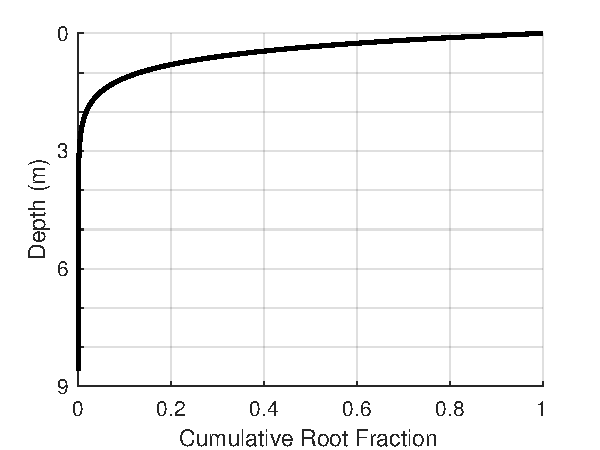
\includegraphics[width=20pc]{../figs3/roots.pdf}
     \caption{Cumulative rooting distribution}
     \label{roots}
  \end{figure}

%====================
%  RESULTS
%====================
\section{Results}  
\subsection{Vegetation water potential}

    PHS introduces prognostic vegetation water potential to CLM at four locations within the plant structure: at the root, stem, shaded leaf, and sunlit leaf.
    Under ambient conditions, 2003 dry season (September-October-November) model average sunlit leaf water potential is -1.65 MPa at midday (local time 12-14h, Figure \ref{fig:vwp}a). 
    The midday pressure drop is primarily between $\psi_{root}$ and $\psi_{stem}$, representing the root collar and upper stem, respectively.
    Under TFE, model midday leaf water potential decreases to -2.31 MPa (Figure \ref{fig:vwp}b). 
    Partitioned among the segments of the SPAC, the change in leaf water potential (totaling -0.66MPa) due to TFE is:
    -0.44MPa soil potential,
    -0.66MPa soil-to-root,
    +0.45MPa root-to-stem, and 
    -0.001MPa stem-to-leaf.
    This comports with previous evidence that seasonal changes in hydraulic resistance are larger belowground \citep{fisher2006}.
    
    Modeled root water potential values match wet season observations, but are less negative than dry season observations under ambient conditions \citep{fisher2006}.
    Midday leaf water potential features a seasonal cycle, with lower values during the dry season (Figure \ref{fig:vwp}c).
    Modeled leaf water potential values under ambient conditions are less negative than averages reported by \cite{fisher2006} (1.71 MPa during the wet season and -2.47 MPa during the dry season), but are within the range of observations.
    The model seems to underestimate isohydricity in response to TFE, showing a drop in leaf water potential of 0.66MPa (dry season, 2003), whereas observations showed no significant difference.


\subsection{Stress factor}
    
    Average midday stress values are comparable during the 2003 dry season (Figure \ref{fig:stress1}) with the two model configurations.
    Under ambient conditions, the average stress factor values are 0.59 and 0.54 for SMS and PHS, respectively (dry season, midday), 
    decreasing to 0.16 and 0.21, with TFE.
    While the SMS stress factor has minimal diurnal variability (Figure \ref{fig:stress1}a),
    PHS features increased stress at midday (Figure \ref{fig:stress1}b), tracking the drop in leaf water potential (Figure \ref{fig:vwp}b,c).
    Likewise, the PHS stress factor responds to both soil moisture and VPD (Figure \ref{fig:stress2}c,d), while SMS responds only to soil moisture (Figure \ref{fig:stress2}a,b).
    This results in more wet season (FMA) stress with PHS (as compared to SMS) under both ambient and TFE conditions (Figure \ref{fig:gpp}a-d).

\begin{table}
\caption{Root-zone soil potential $^a$ (MPa) terciles for Figure \ref{fig:stress2}}
\label{tab:tercile}
\centering
\begin{tabular}{c c c }
Simulation & T1 & T2 \\
\hline
SMS, Ambient & -0.01 & -0.54 \\
SMS, TFE & -0.29 & -1.74 \\
PHS, Ambient & -0.01 & -0.05 \\
PHS, TFE & -0.05 & -0.33 \\
\hline
\multicolumn{2}{p{.5\linewidth}}{$^{a}$SMS values correspond to daily mean root-fraction weighted soil potential.
PHS values correspond to predawn root water potential.}
\end{tabular}
\end{table}


\subsection{GPP and Transpiration}
    The two models predict similar total GPP across 2002-2003 under TFE, 3.96 kg/m$^2$ (SMS) and 4.00 kg/m$^2$ (PHS), 
    but GPP is lower for PHS under ambient conditions (4.86 kg/m$^2$) as compared to SMS (5.46 kg/m$^2$, Figure \ref{fig:gpp}e-h).
    Seasonal variability in GPP is smaller with PHS. 
    The standard deviations of daily GPP (2002-2003) are 0.49 and 1.55 g/m2/d for AMB/TFE, 
    as compared to 1.53, 2.73 g/m2/d with SMS. 
    Transpiration seasonality is featured in both models (Figure \ref{fig:t}a,b), but with a larger amplitude for SMS.
    PHS yields a better fit to field observations of daily sap flux (see Section zqz), with higher R$^2$ and lower RMSE compared to SMS 
    under both ambient and TFE conditions (Figure \ref{fig:t}c-f).

    
\subsection{Hydraulic conductance}
    The two model configurations differ in how to impose the diurnal cycle in root water uptake (Figure \ref{fig:cond}).
    With PHS, the diurnal cycle features in the gradient in water potential from $\psi_{\text{soil}}$ to $\psi_{\text{root}}$,
    while with SMS, $\Delta\psi$ features no diurnal variability on average (Figure \ref{fig:cond}c).
    Instead SMS imposes a diurnal cycle through hydraulic conductance (Figure \ref{fig:cond}a).
    In response to TFE, PHS features an increase in $\Delta\psi$ compared to a decrease with SMS.
    Alternatively, hydraulic conductance decreases with TFE with PHS, but increases under SMS.
    Both models net a decrease in root water uptake under TFE.
    
    PHS conductance is modeled based on xylem vulnerability and Brooks-Corey, 
    imposing a strong dependence on soil potential (Supp Fig \ref{supp:cond2}a).
    

\subsection{Root water uptake}
    dry-amb, comparable total transpiration (phs:28.3, sms:28.5cm)  but distinct profiles, PHS removes less water from intermediate soil layers (0.5-1.5meters) (Figure \ref{fig:qdry}d),.
    Partitioning between surface and beyond more sensitive to precipitation with PHS (Figure \ref{fig:qdry}a-c).
    Both models decrease surface extraction with TFE (Figure \ref{fig:qdry}b), but PHS has a larger compensation from depth (Figure \ref{fig:qdry}c),
    allowing more overall transpiration (14.6 vs. 10.8 cm).
    
    Wet season PHS opts for surface water, with zero net extraction beyond [35.2,9.6cm].
    SMS for reference extracts [49.8\%,81.5\%] of water from down there (Figure \ref{fig:qwet}). 
    PHS does extract farther into the soil profile, but in service of HR, 
    sending surface water to depth.
    PHS can achieve higher root water uptake rates, especially under wet conditions, where, for example, 
    Soil Layer 2 dries much faster than with the SMS formulation after rain events (Supp Fig \ref{supp:layer2})
        
\subsection{Hydraulic redistribution}
    HR totals to [38.9/40.0] with the majority occurring at night [28.0/26.7] (Figure \ref{fig:hr}).
    Total HR refers to the sum of all reversed flows, namely from root-to-soil.
    Note that over the course of a day or season, HR can occur without net negative root water uptake.
    For example, hydraulic lift may occur at night, moving water from deep in the soil column up to near the surface, which is then more readily available for transpiration during the following day.    

    Different seasonality AMB has more HR during Sept-Jan, TFE during Feb-Apr.
    HR occurs in both directions (Supp Fig \ref{supp:hr}), but is predominately downwards [30.65/33.75].

\subsection{Soil moisture}
    During the dry season, SMS simulations yield much lower values for soil matric potential (Figure \ref{fig:sm}, Supp Fig \ref{supp:sm}). 
    The average soil potential  is -1.42 MPa during SON under ambient conditions, as compared to -0.14 MPa in the PHS simulation.
    With TFE, SMS is -2.51 MPa and PHS is -0.5 MPa.
    Following from the definitions of root water uptake (see Section zqz), we use different methods for calculating average soil potential.
    With SMS we utilize root-fraction weighted averaging.
    With PHS we opt for predawn (5h) root water potential. 

    PHS better matches observations, especially in the top meter of the soil column, with RMSE lower by up to 55\%.
    SMS seems to pull too hard in 0-0.3m, 0.5m, and 1m, with soil potential too low during the dry season.
    This is associated with the soil wilting parameter ($\psi_c$), which takes the value -2.5MPa for BET \citep{oleson2013}.
    It is not a coincidence that this value is equivalent to SMS TFE smp average in the last paragraph.
    Root water uptake depends on $\psi_c$, with this parameter serving as the lower bound for soil potential 
    (except in the first two soil layers, which are under the influence of soil evaporation).
    Beyond 1m, root fractions are smaller, attenuating the dry bias.
    
\subsection{Soil moisture effect on transpiration}    
    Model soil potential shows limited effect on transpiration in the ambient simulations, 
    based on sap flux observations (Supp Fig \ref{supp:cool}b,f).
    However, in the SMS configuration, modeled transpiration decreases with more negative soil potential (Supp Fig \ref{supp:cool}a),
    biasing the model relative to observations (Fig \ref{fig:cool}a).
    
    Observed transpiration under TFE shows a stronger relationship with soil potential in the 
    PHS simulation than in the SMS simulation (Supp Fig \ref{supp:cool}h,d).
    And again the relationship with soil potential seems to bias modeled transpiration with SMS (Fig \ref{fig:cool}b).
    The two PHS simulations feature less structure in transpiration bias vs. soil potential and less bias overall (Fig \ref{fig:cool}c,d).


    
\section{Discussion}
\subsection{The promise of plant hydraulics}
    Plant hydraulics have promised to improve model predictions of vegetation response to climate change \citep{sperry2015}, 
    especially if parameter ranges and model complexity can be constrained \citep{rogers2017}.
    Numerous site-level models have deployed plant hydraulics (e.g. \citet{williams1996,sperry1998,bohrer2005}), and studies show
    vegetation water potential can improve predictions of stomatal response to the environment \citep{sperry2017,anderegg2017},
    More recently hydraulics have been coupled to global models \citep{bonan2014,xu2016,christoffersen2016}, 
    but most Earth System Models do not provide mechanistic representation of vegetation water dynamics.

    In this study, we implement plant hydraulic theory within CLM5, 
    using vegetation water potential to modulate leaf gas exchange and root water uptake.
    We model water potential according to a simplified circuit analogy (Figure \ref{circuit}), which captures expected diurnal and seasonal dynamics of leaf water potential (Figure \ref{fig:vwp}).
    Under ambient conditions hydraulic resistance is largest from root-to-stem (Figure \ref{fig:vwp}a), 
    while the added resistance from TFE is primarily from soil-to-root (Figure \ref{fig:vwp}b), consistent with previous results \citep{fisher2006}.

    Support for hydraulic models cites possible improvements in modeling mortality and productivity \citep{mcdowell2018,choat2012}.
    However, concerns exist in the literature regarding hydraulic model complexity and parameterization \citep{verhoef2014,drake2017}, 
    which informed our model design (see Section zqz).
    Recent work suggests model complexity can be managed, with significant coordination of hydraulic traits \citep{bartlett2016,christoffersen2016}.
    Likewise incorporating plant hydraulics provides access to new streams of observational data for model validation.
    Vegetation water potential can be monitored in the field \citep{boyer1967} and has been shown to correlate with remote sensing products \citep{momen2017}.
    Parameter values can be measured in the field \citep{sack2002} and are available in the TRY database \citep{kattge2011}.

\subsection{Water stress and stomatal conductance}

    PHS models sunlit and shaded leaf water potential, which serve as the functional input to the water stress factor, 
    replacing the previous version based on soil water potential.
    This imparts a diurnal cycle to the water stress factor (Figure \ref{fig:stress1}), following the midday drop in leaf water potential.
    As such, stress now depends on transpiration demand, and, in turn, VPD and solar radiation (Figures \ref{fig:stress2},\ref{supp:fsds}).
    Medlyn does already reduce stomatal conductance based on VPD, but based on A-$\lambda$E.
    Here we are trying to impart xylem tension stress, allowing plants to avoid cavitation and embolism.
    Support for this in the literature \citep{novick2016a,sperry2017}, but still no consensus on the best functional form \citep{zhou2013}. 
    
    The water stress factor follows a seasonal cycle, with lower (indicating more stress) values during the dry season, 
    but with less seasonal variation compared to the control model (Figure \ref{fig:gpp}a-d).
    As a result PHS features less seasonal variability in GPP, especially under ambient conditions (Figure \ref{fig:gpp}e-h).
    The xylem tension constraint in PHS imparts a negative feedback on GPP.
    Factors increasing GPP (e.g. more light) also increase xylem tension and stress, which limits GPP.
    \cite{restrepo2017} show that GPP increases at Caxiuana during the dry season, suggesting that PHS improves the GPP seasonal cycle relative to the control model.
    
    PHS underestimates the seasonal cycle in transpiration under ambient predictions, with less variability than sap flux observations (Figure \ref{fig:t}a,c).
    Likewise, we produce a high bias in transpiration under TFE, similar to previous evidence showing that models tend to underestimate the effect of TFE \citep{powell2013}.
    Considerable uncertainty remains regarding the appropriate functional form of water stress.
    Further work could examine other permutations of water stress, and/or concurrent improvement in photosynthesis parameters and model structure.
    While a work in progress, PHS does improve transpiration predictions, 
    with lower RMSE and higher correlation compared to the control model, albeit with model tuning (Figure \ref{fig:t}).
    
\subsection{Structural improvements in modeling root water uptake}
Our pull evolves in time
Our conductance responds to soil moisture
\subsection{HR}
\subsection{Soil moisture and its influence on transpiration}

    
\section{leftovers from previous version}
    
 This is consistent with findings in \cite{fisher2006} that most of the whole-plant resistance is above ground, but that added resistance from drying is predominately sourced? below ground. Likewise \cite{fisher2006} found evidence of isohydric behavior, where plants manage water loss through stomata to regulate leaf water potential, which is consistent with results here of reduction in potential drop across the stem. However, PHS shows declines in midday leaf water potential due to TFE, but \cite{fisher2006} found no significant observed difference between ambient and TFE dry season leaf water potential. This could indicate that our parameters do not result in sufficiently isohydric behavior.
    
    Many facets of our hydraulic representation are simplified relative to the literature, reflecting that in a model designed to operate at the global scale,  there is a tradeoff between added complexity and parameter reduction. The current PHS parameterization omits vegetation capacitance,  which may be important for accurately modeling the diurnal cycle of water stress especially in tropical rainforests \citep{meinzer2009}. Further, hydraulic conductance hysteresis and permanent cavitation are absent from the PHS vulnerability parameterization, whereby xylem segments fully regain conducting capacity upon re-wetting. This limits the influence of drought legacy, which has been shown to be significant for forest mortality \citep{anderegg2013}.
    
    Similar to other simplified models \citep{xu2016}, loss of conductance is based on lower terminus water potential, which may underestimate integrated loss of conductivity \citep{sperry2015}. These simplifications each serve to lessen the parameter and/or computational burden of PHS. Our objective was to simplify the plant hydraulic representation for this initial implementation, acknowledging that more comprehensive process representation may prove necessary for future model versions.

\subsection{Stress factor, annual dynamics}

In the dry season surface drying also decreases soil-root conductance so that it is easier to extract moisture from deeper layers, consistent with observations based on isotopes (CITATION).
Observations indicate the trees here adopt an isohydric behavior, where declines in soil moisture are tightly coupled with reduced transpiration, which mitigates decreases in leaf water potential \citep{fisher2006}. The parameter values employed for these simulations may be insufficiently isohydric (GIVE REFERENCE AND DEFINE ISOHYDRICITY), which could explain limited sensitivity to TFE relative to observations.
    
    Water stress is applied to capture limitations with declining water status that are not reflected within the Medlyn stomatal optimization theory (which only optimizes $\delta E / \delta A$, and thus does not take water supply into account). CLM implements non-stomatal limitation by multiplying $V_{\text{cmax}}$ by $f_w$. Though there is limited evidence of down-regulation of $V_{\text{cmax}}$ \citep{flexas2006}, this was the best option within CLM  for applying stress through the GPP term of the stomatal conductance model, in accordance with field observations \citep{lin2018,zhou2013}.
    If in future versions of CLM, mesophyll conductance is represented, it may be a more appropriate avenue for achieving the same effect. (MERGE WITH PREVIOUS DISCUSSION, TRY AVOIDING REPETITIONS A MUCH AS POSSIBLE)
    
    Given constant stomatal conductance, xylem tension increases with declining soil water, but also with increasing vapor pressure deficit.
    While VPD sensitivity is included in the Medlyn model, it serves to mitigate increasing water costs, without consideration of cavitation.
        Total soil water content (or departure from saturation) is a typical basis for diagnosing water status and stress \citep{drake2017}, which is in line with an SMS-type approach.
    While capturing supply limitations, this framework neglects effects of transpiration demand on xylem tension.
    Evidence suggests that vegetation employ water use strategies to mitigate the risk of cavitation associated with increasing xylem tension \citep{sperry1998,fisher2006,choat2012}.
    Utilizing leaf water potential as the basis for water status reflects this constraint.
    This may be especially important given projected increases in VPD associated with warming.

\subsection{Hydraulic redistribution}

    During the wet season surface extraction supplies transpiration, but is also redistributed into lower soil layers. Hydraulic redistribution has been observed in the field \citep{oliveira2005}, and is not represented in the SMS version of the CLM \citep{lee2005}. which sets root water uptake to zero if the gradient in water potential is negative. 
    
    For HR to occur into a soil layer, the soil potential must be more negative (drier) than the $\psi_{\text{root}}$ (see Figure . During the day, transpiration requires a gradient in water potential from soil-to-root, which lowers $\psi_{\text{root}}$, decreasing the amount of HR.Therefore, in PHS, more HR occurs at night, in accordance with observations and theory \citep{oliveira2005,lee2005}.
    
    HR is predominately downwards during the wet season (FMA), serving to diminish the gradient between the newly-wetted surface and still-dry depths (Supp Figs A.6,A.7). Redistribution occurs in both directions during the dry season (SON), downwards after rain events, and upwards with drying. Only with TFE, and only during the dry season, is there significant extraction beyond 6 meters (Figs 8, 9). There is very little water deposited at depths beyond 6 meters at any point in either simulation.

    
    The dynamics of HR with PHS align with observations, with more HR at night, and HR occurring in both directions vertically \citep{burgess1998}.
    The absolute values of HR are difficult to assess, given limited observations.
    
    In PHS, Allowing HR to occur into the top layer of the soil column significantly degraded modeled soil evaporation (not shown). We opted to omit the first top Layer (spanning 0 to 2 cm below ground) soil-to-root hydraulic conductance, to prevent HR from over-supplying water for soil evaporation.
    
\subsubsection{Is hydraulic redistribution a feature or a liability?}
   
    HR is a natural consequence of using Darcy's Law to model root water uptake - when hydraulic gradients are reversed, HR should occur. As such it is naturally included within a plant hydraulics model with multiple soil layers and is an emergent behavior of respecting hydraulic flow down gradient of potentials.  In ESMs, where soil moisture is typically resolved vertically, interfacing the plant hydrulics with a multi-layer soil naturally accounts for HR. Other models, similar to the SMS paradigm, disallow HR by constraining root water uptake to be positive \citep{xu2016}.
    
    Most literature models force the model with a single bulk soil water potential $\psi_s$, which precludes HR \citep{fisher2007,bonan2014,sperry2017}. \cite{christoffersen2016} expand beyond a single $\psi_s$ horizontally, representing soil elements at different charecteristic distances from the root surface,  but still feature a single soil layer in the vertical dimension.  
    
    Likewise HR is likely sensitive to the representation of vegetation tissue capacitance and below-ground hydraulic segmentation (CITAIONS NEEDED).
    
    Hydraulic redistribution has the impact of reducing the variance in the availability of water for plant transpiration, potentially at odds with observations of interannual variation (see Lawrence et al in prep. Tang et al. 2015) Observations of HR are extremely difficult, in unequivocal detection of HR involves the observation of reverse flow along transport roots, typically at rates close ot the detection threshold of sap flow monitoring systems. Therefore, the degree to which HR actually occurs in unclear. While there is some first-order benefit to plants of moving water from deep soil to surface layers to allow more transpiration, this water is then also available for competition with other shallow-rooted plants, and for evaporative processes. Further, cavitation of fine roots in shallow soils might explicitly act as a 'fuse' to prevent loss of water from the plant into dry soil layers (Kotowska et al. 2015) - a process not explicitly resolved here. Therefore we view this first implementation of HR into the default versions of the CLM as a 'null' hypothesis for the functioning of this process, and as a platform to allow further refinement from the plant hydraulics community. 
    

\section{Conclusion}

\subsection{Caveats}

    Modeling stomatal conductance and photosynthesis, especially subject to water stress, is an area of ongoing research. We use the Medlyn model coupled to a hydraulic stress function that attenuates $V_{\text{cmax}}$. This complies with observations \citep{lin2018,zhou2013} that stress applied through $g_1$ underestimates attenuation of photosynthesis. However, there is no direct evidence of declines in $V_{\text{cmax}}$ with drought \citep{flexas2006}, whereby future work may seek to represent mesophyll conductance in CLM.
    
    The model hydraulic supply representation is simplified, to reduce the model parameter and computational burdens.
    No capacitance.
    No integration of xylem or soil conductances vulnerability, instead based on lower node.
    No hysteresis in loss of conductance, xylem instantly regain conductance upon re-wetting.
    Leaf conductance simplified.
    Soil layers fully parallel, soil potential constant each time step.
    
    Parameter uncertainty is significant.
    Notions of hydraulic architecture will never perfectly fit on this modeling scale, especially in a PFT paradigm.
    Field measurements of hydraulic traits will help constrain parameter ranges, but mostly only aboveground.
    Flux observations can help to tune stress parameters.
    Parameter estimation for root functioning is significantly more challenging, given the difficulty in underground trait observations.
    Likewise observational constraints of vertically-resolved states and fluxes underground are scarce.
    Follow-up work will be geared towards parameter estimation and assessing model skill.

\subsection{Utility of modeling vegetation water potential}


    The PHS configuration of the CLM5 is, to our knowledge, the first Earth System Model with a representation of plant water potential running in its default configuration. In this paper, we have described the model implementation, and illustrated a comparison of the model dynamics for a tropical rainforest site subjected to water limitation, given that prediction of rainforest responses to drought is one of the key uncertainties in the ESM predictions. Overall, the new model behaviour differs from the default configuration in ways that are expected, given its structural properties, and in many cases, provides better correspondance with the observations that the default structure. 
    
    In this paper, however, we do not undertake a comprehensive assessment of which model structure performs better, given the substantial parametric uncertainty in both models, and the dependence on numerous other features of the CLM external to water stress representation that contribute to model-observation divergences - in this case in particular, the overestimation of unstressed transpiration by both versions of the model compared to the observations. 
    
    In lieu of this type of assessment, we propose that the new PHS model structure 1) is more closely aligned with known plant hydraulics theory, 2) provides significantly improved connections to real-world observational data streams (of leaf and stem water status, sap flow, percent loss conductance) and 3) represents known features of ecohydrological function that the default model cannot capture, including hydraulic redistribution, changes in the depth of water uptake with drought stress, plant embolism impacts on gas exchange and responses of water uptake to changes in leaf:root rations. 
    
   
    This will be the final conclusions.
    Any comments on overall takeaways?

    PHS models vegetation water potential. 
    This offers structural improvements for stress and for root water uptake.
    Stress now functions with hydraulic limitation.
    
    

\section{Acknowledgments}

\clearpage    

\section{Figures}
  \begin{figure}[h]
     \centering
     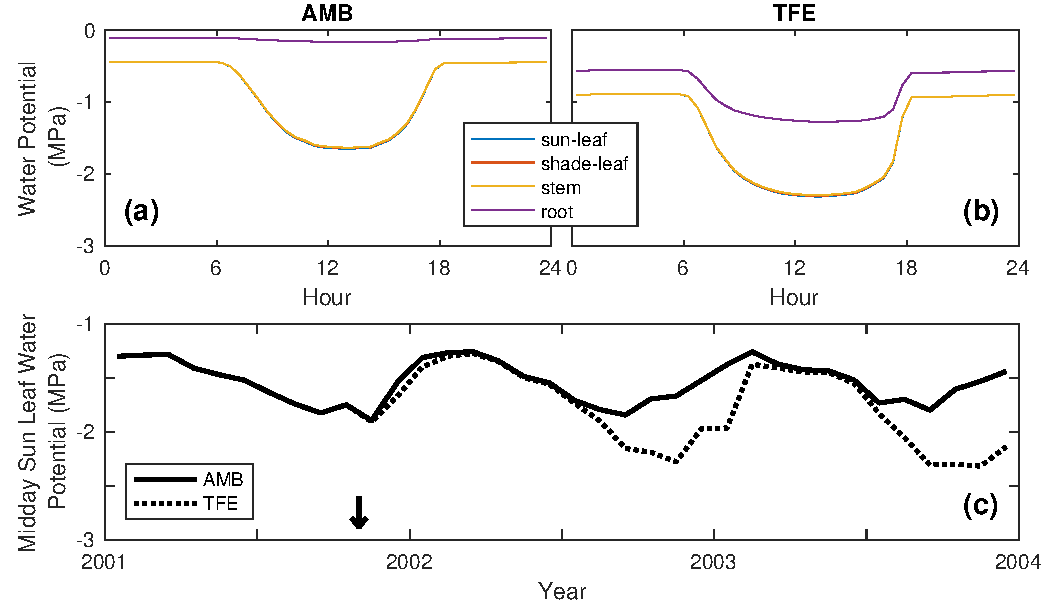
\includegraphics[width=30pc]{../figs3/vwp.pdf}
     \caption{Modeled vegetation water potential at  Caxiuan\~a, Brazil.
     (a) 2003 dry season (SON) diurnal mean, ambient through-fall conditions,
     (b) 2003 dry season diurnal mean, with 60\% TFE.
     Curves are drawn for sunlit leaf, shaded leaf, stem, and root water potentials, with the first three mostly overlapping.
     (c) Monthly average midday (12h-14h) leaf water potential, under ambient (solid line) and TFE (dotted line) conditions.
     Note that TFE begins Nov 1, 2001, as indicated by the vertical arrow. 
     }
     \label{fig:vwp}
  \end{figure}

  
    \clearpage
    \begin{figure}[h]
     \centering
     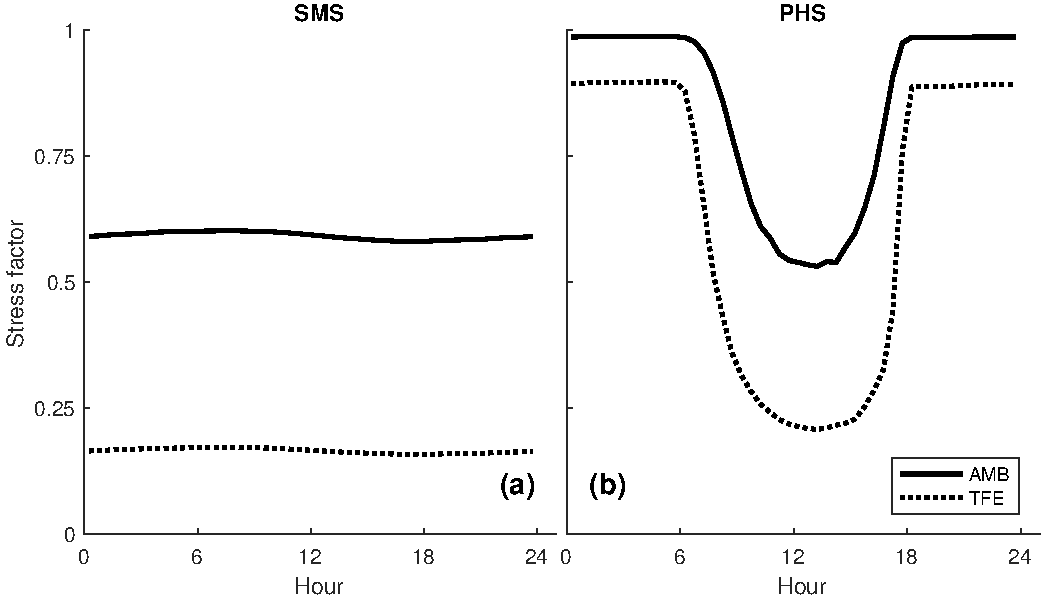
\includegraphics[width=30pc]{../figs3/fig4.pdf}
     \caption{2003 dry season (SON) diurnal mean water stress function for 
     (a) SMS, and
     (b) PHS.
     Note that the water stress factor equals 1 when there is no stress and 0 when fully stressed.
     }
     \label{fig:stress1}
  \end{figure}
  
      \clearpage
    \begin{figure}[h]
     \centering
     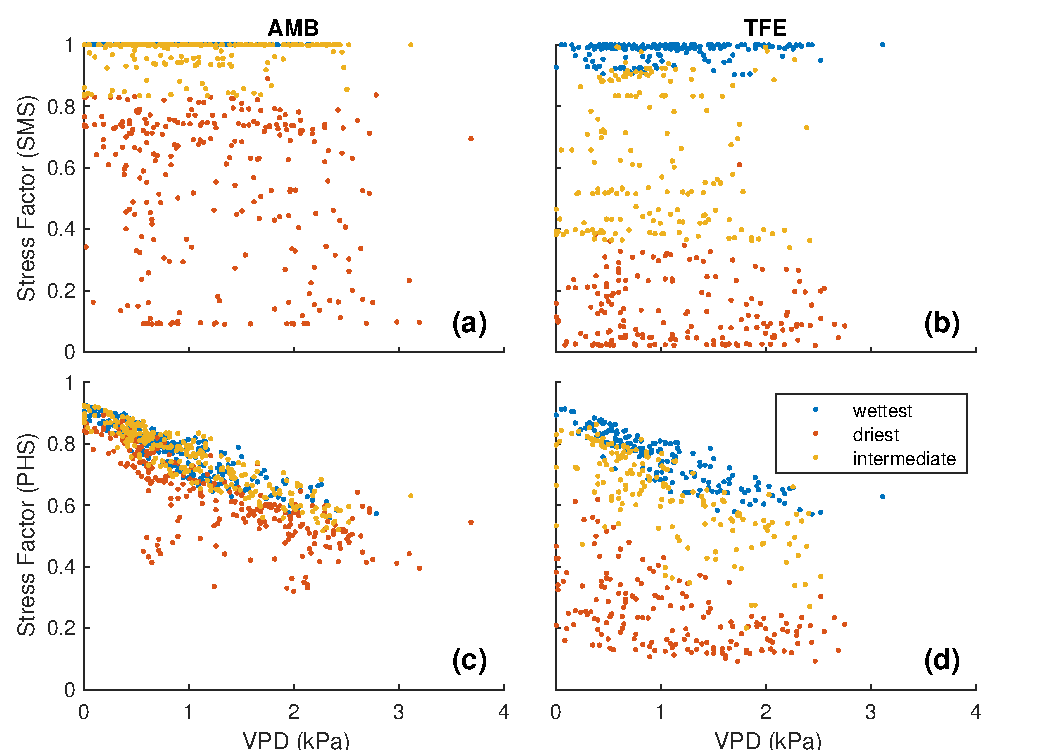
\includegraphics[width=30pc]{../figs3/vpdstress.pdf}
     \caption{Water stress factor versus vapor pressure deficit (2002-2003), for timesteps with downwelling shortwave radiation between 400 and 425 W/m2 (n=515).
     Radiation is controlled to highlight the relationship with VPD, the reverse (controlling for VPD) is shown in Figure \ref{supp:fsds}.
     For SMS (a,b), data are subdivided based on average soil matric potential, weighted by root fraction.
     For PHS (c,d), data are subdivided based on predawn (5h) root water potential.
     Blue dots represent the wettest tercile, yellow dots represent the intermediate tercile, and red dots represent the driest tercile (see Table \ref{tab:tercile}).
     }
     \label{fig:stress2}
       \end{figure}
      
          \clearpage   
  \begin{figure}[h]
     \centering
     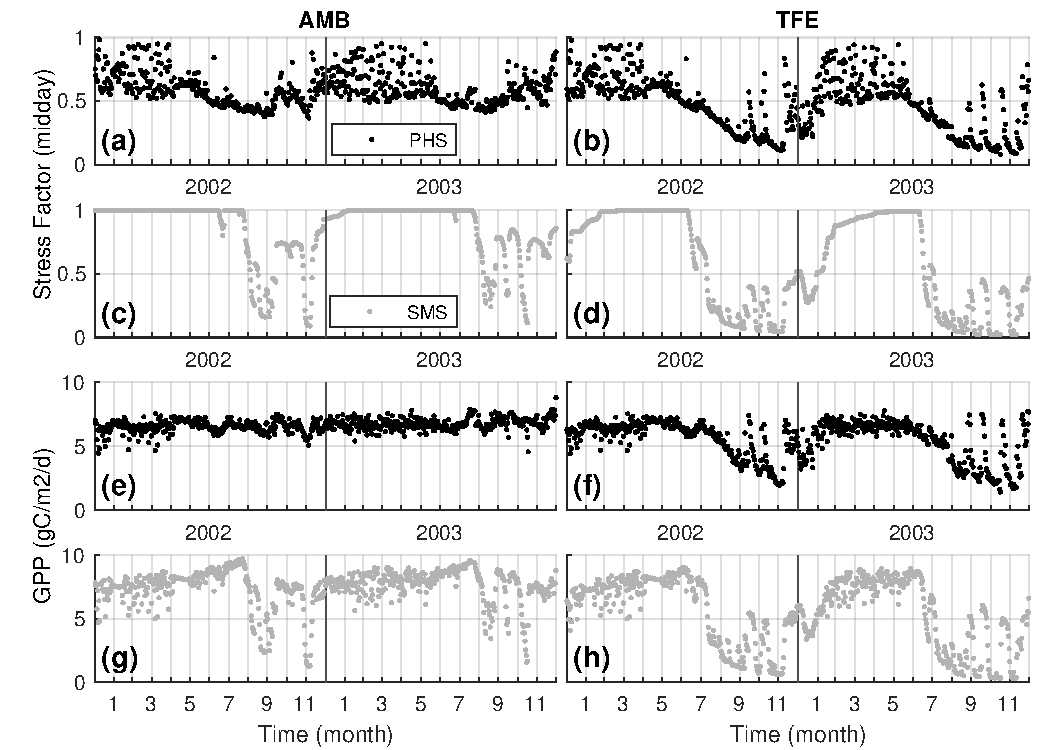
\includegraphics[width=30pc]{../figs3/gpp.pdf}
     \caption{Daily stress factor (midday, averaged over 12h-14h) and GPP during 2002-2003 under ambient (left) and TFE (right) conditions.
     Output from the SMS configuration (a,b,e,f) are plotted with gray color, while output from the PHS configuration (c,d,g,h) are plotted in black.
     }
     \label{fig:gpp}
  \end{figure} 
         
  \clearpage   
  \begin{figure}[h]
     \centering
     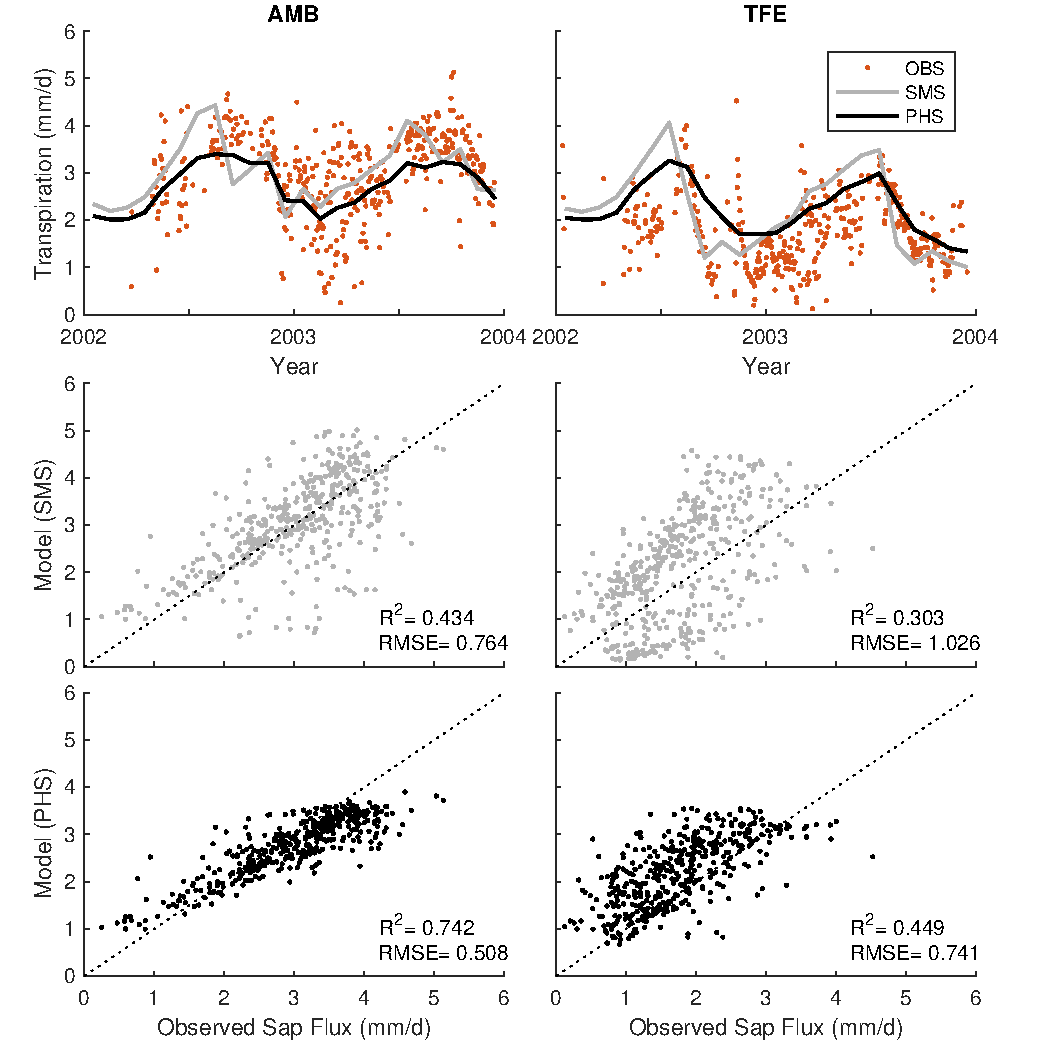
\includegraphics[width=30pc]{../figs3/T.pdf}
     \caption{(a,b) Monthly mean water stress function. The water stress factor equals 1 when there is no stress and 0 when fully stressed.
     (c,d) Monthly mean transpiration (W/m$^2$).
     (e,f) Monthly mean gross primary productivity (g/m$^2$/d). 
     Solid lines correspond to ambient through-fall conditions, and dotted lines feature 60\% through-fall exclusion.
     Black lines represent model output.
     Red lines show observational transpiration derived from sap flux (see zqz).
     PHS is on for (a), (c), and (e). PHS is off for (b), (d), and (f).
     }
     \label{fig:t}
  \end{figure}

\clearpage   
  \begin{figure}[h]
     \centering
     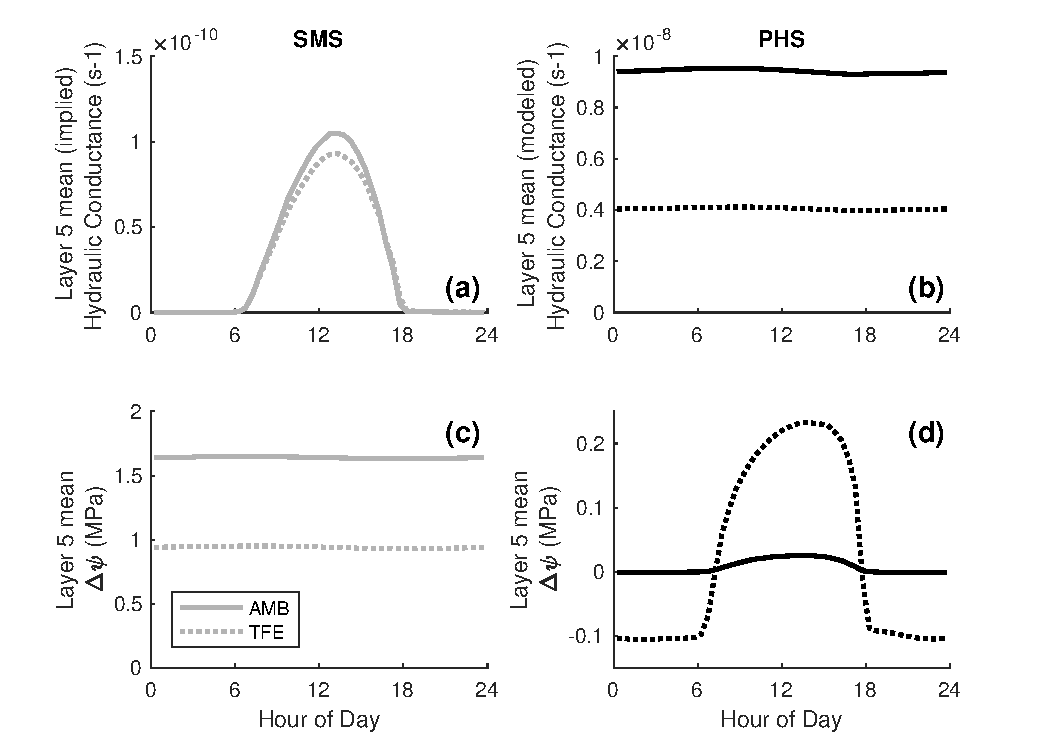
\includegraphics[width=30pc]{../figs3/k.pdf}
     \caption{Diurnal mean of the Soil Layer 5 conductance, under ambient and TFE conditions during 2003. 
     (a) Time-series of PHS modeled soil-to-root conductance (s$^{-1}$) from Soil Layer 5 (spanning 20 to 32 centimeters in depth).
     (b) Time-series of SMS inferred conductance (s$^{-1}$) also from Soil Layer 5.
     }
     \label{fig:cond}
  \end{figure}
  

        \clearpage
    \begin{figure}[h]
     \centering
     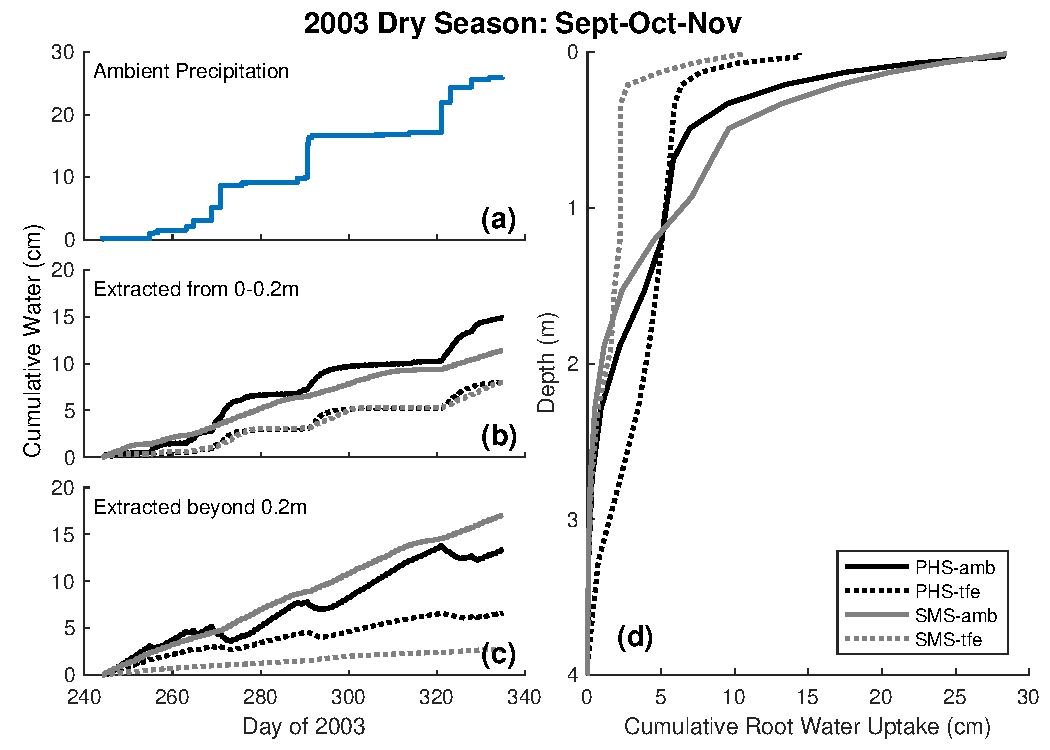
\includegraphics[width=30pc]{../figs3/qdry.pdf}
     \caption{2003 dry season (SON) cumulative root water uptake and precipitation. 
     (a) Cumulative root water uptake with depth across the four simulations.
     (b,c) Cumulative water uptake over time from above and below 0.2m, respectively.
     (d) Cumulative precipitation under ambient conditions.
     }
     \label{fig:qdry}
  \end{figure}
  
        \clearpage
    \begin{figure}[h]
     \centering
     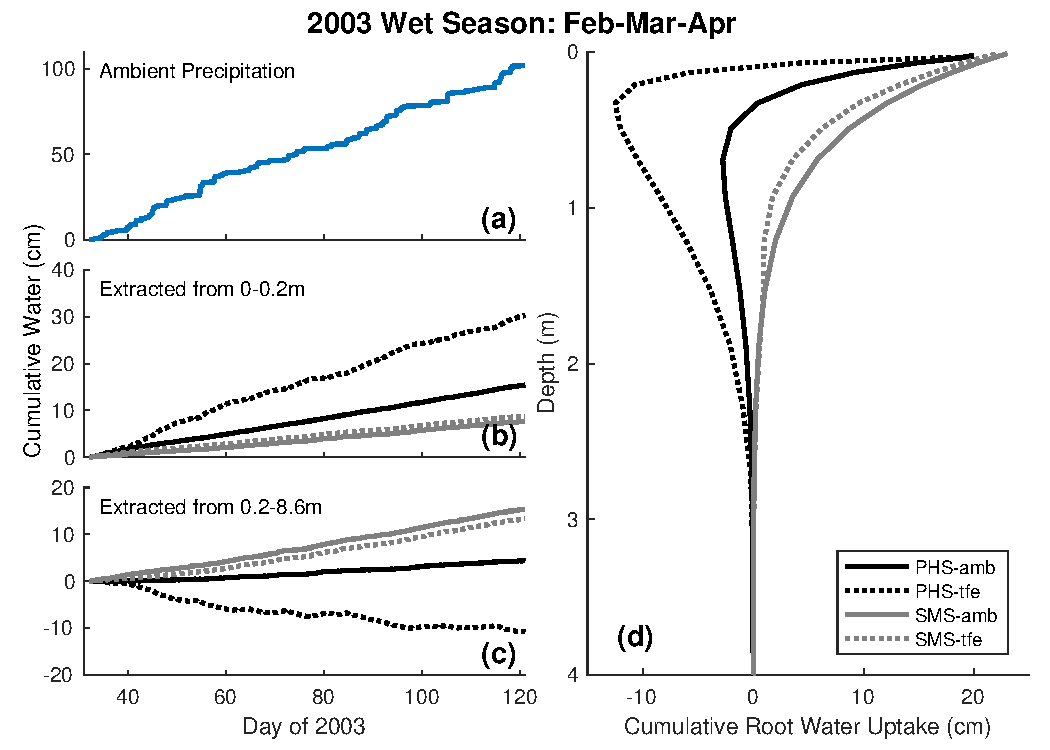
\includegraphics[width=30pc]{../figs3/qwet.pdf}
     \caption{2003 wet season (FMA) cumulative root water uptake and precipitation. 
     (a) Cumulative root water uptake with depth across the four simulations.
     (b,c) Cumulative water uptake over time from above and below 0.2m, respectively.
     (d) Cumulative precipitation under ambient conditions.
     }
     \label{fig:qwet}
  \end{figure}
  
    \clearpage
    \begin{figure}[h]
     \centering
     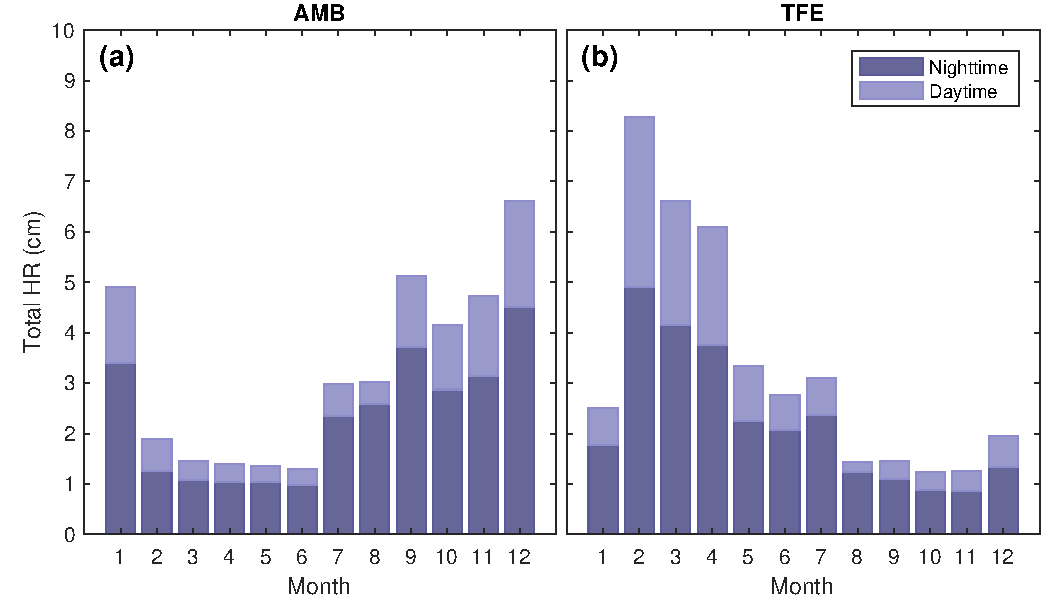
\includegraphics[width=30pc]{../figs3/hr.pdf}
     \caption{Total hydraulic redistribution (cm) by month across in 2003. For (a) ambient through-fall conditions, and (b) 60\% through-fall exclusion. 
     Darker shading shows portion of HR at night [6pm,6am), lighter shading shows portion of HR during day [6am,6pm).}
     \label{fig:hr}
  \end{figure}

  
      \clearpage
    \begin{figure}[h]
     \centering
     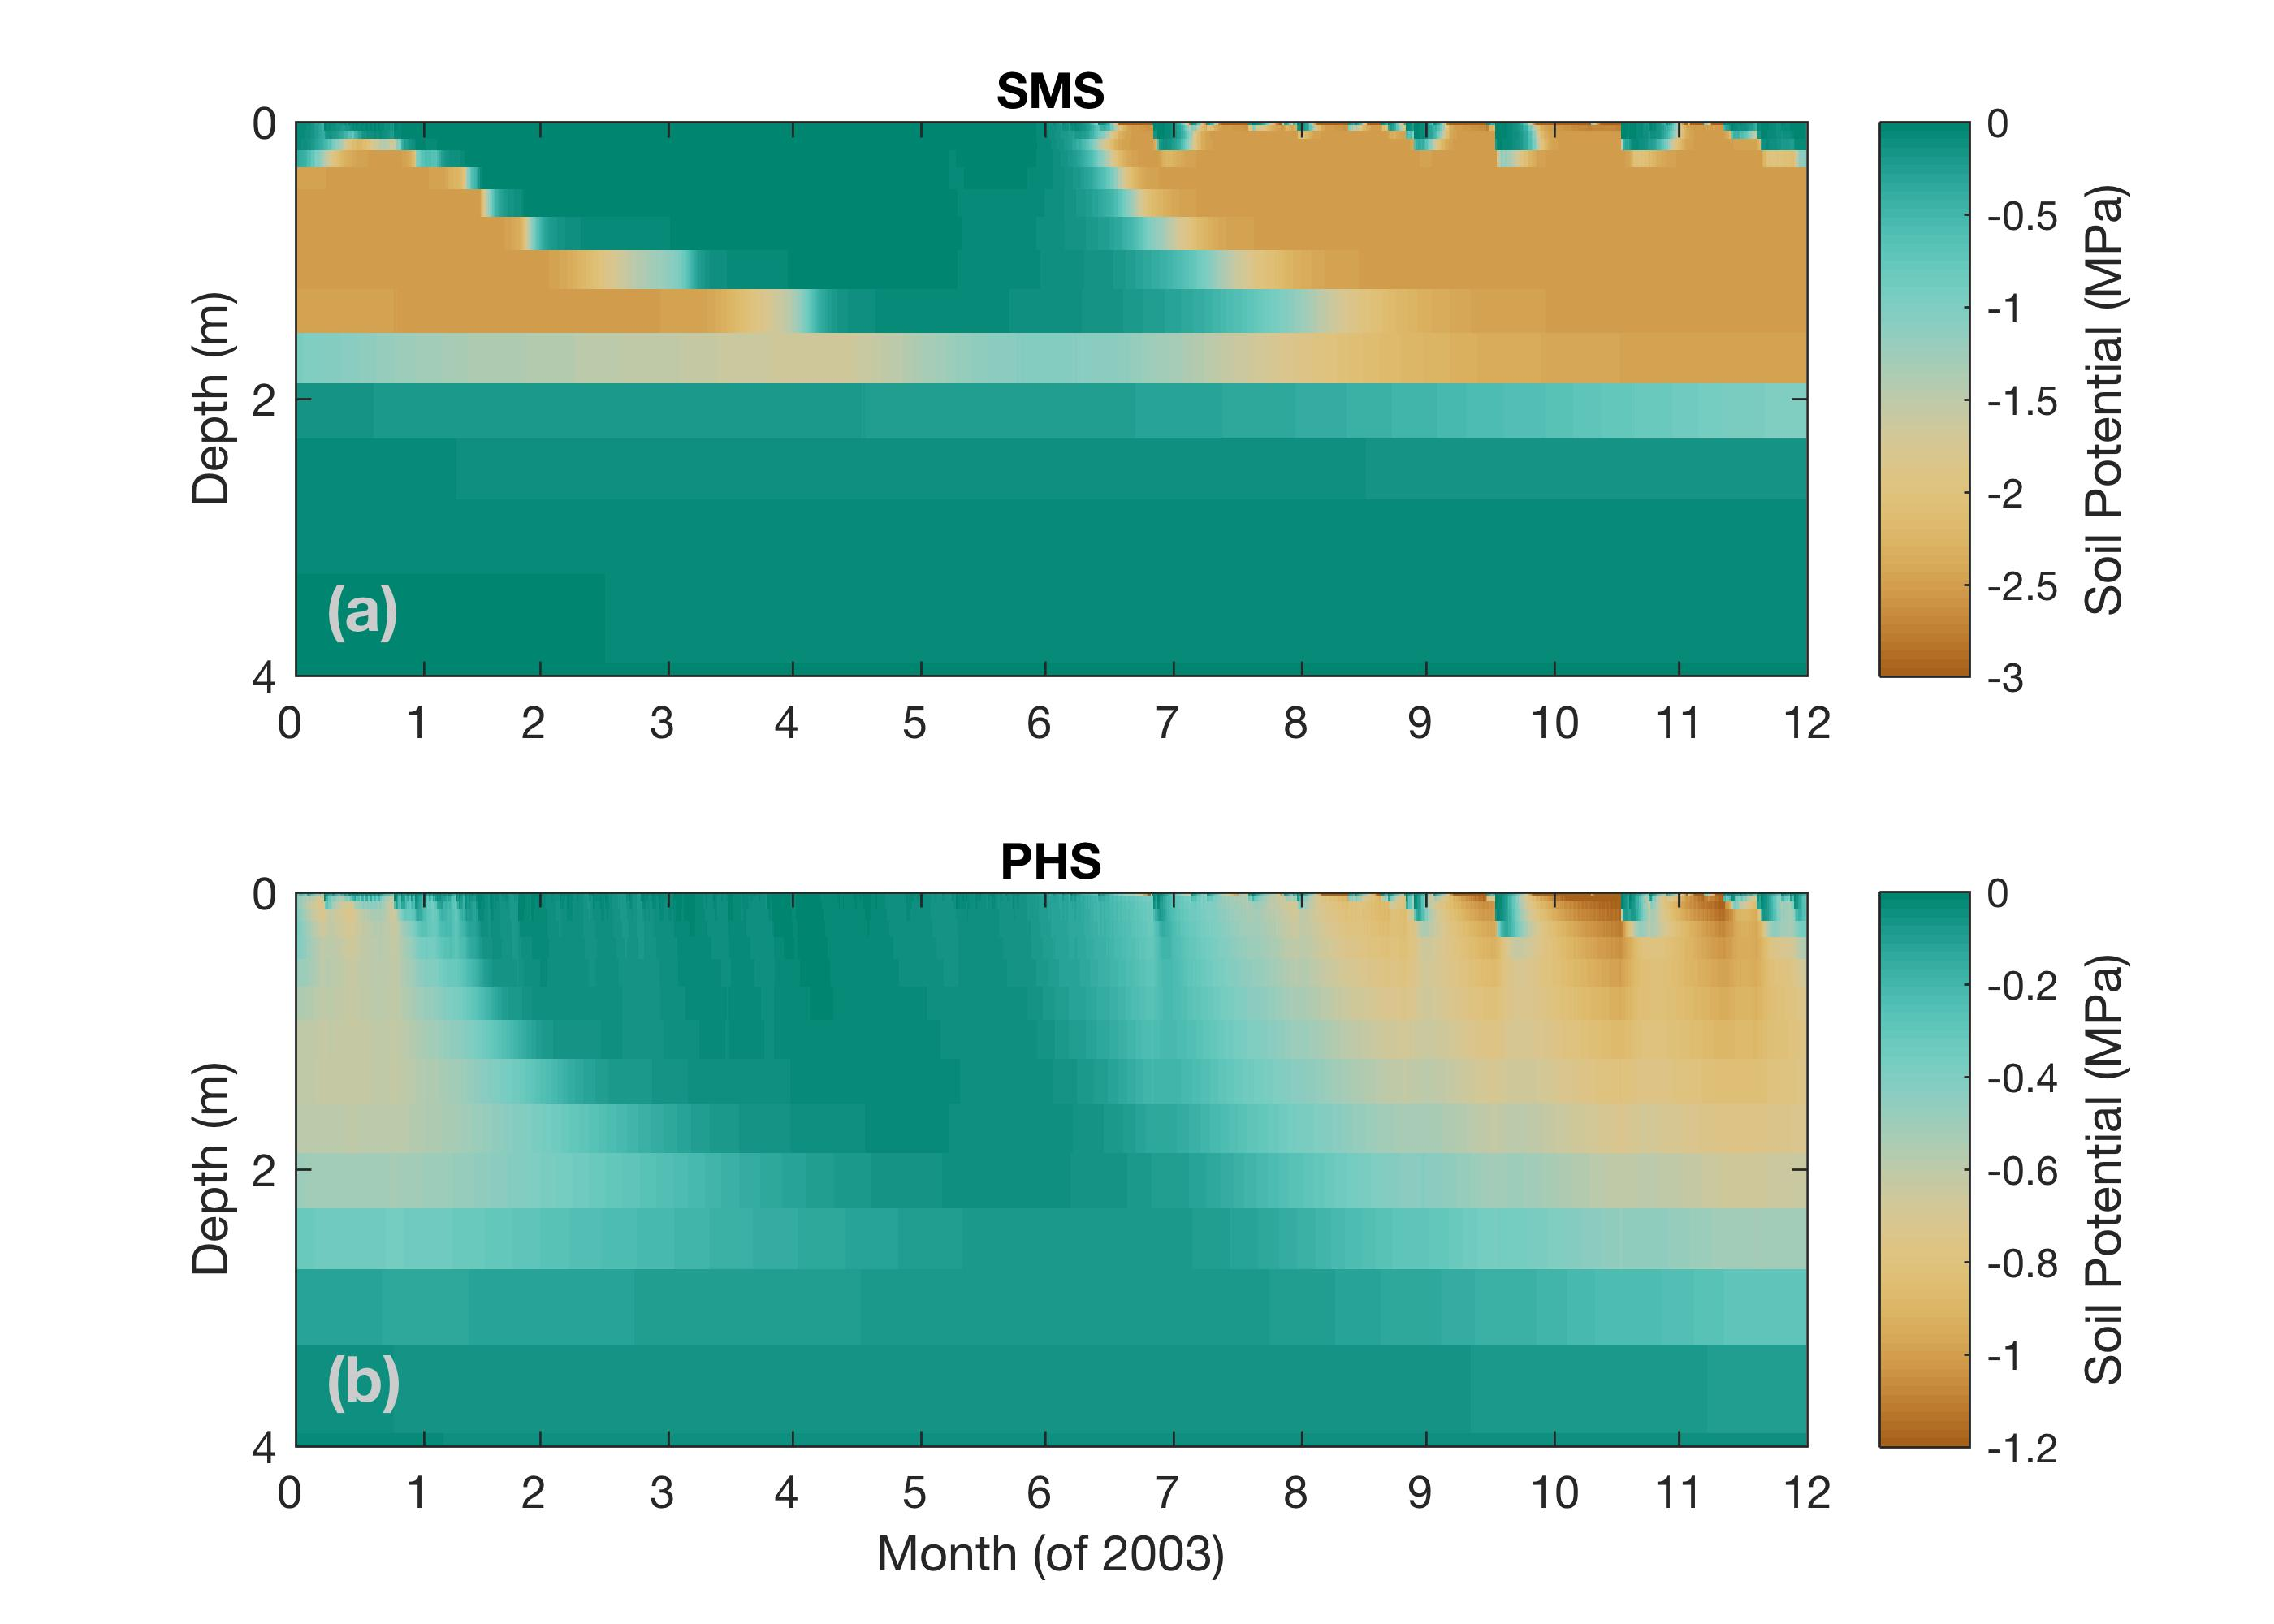
\includegraphics[width=30pc]{../figs3/smp.jpg}
     \caption{Vertical profile of soil water potential (MPa) over time under 60\% through-fall exclusion, for
     (a) PHS, and 
     (b) SMS.
     Note that color axes are different.
     Figure \ref{supp:sm} duplicates this analysis under ambient conditions.
     Figure \ref{fig:sm2} replots this data along with observational soil moisture at 0.5m depth. }
     \label{fig:sm}
  \end{figure}
  
        \clearpage
    \begin{figure}[h]
     \centering
     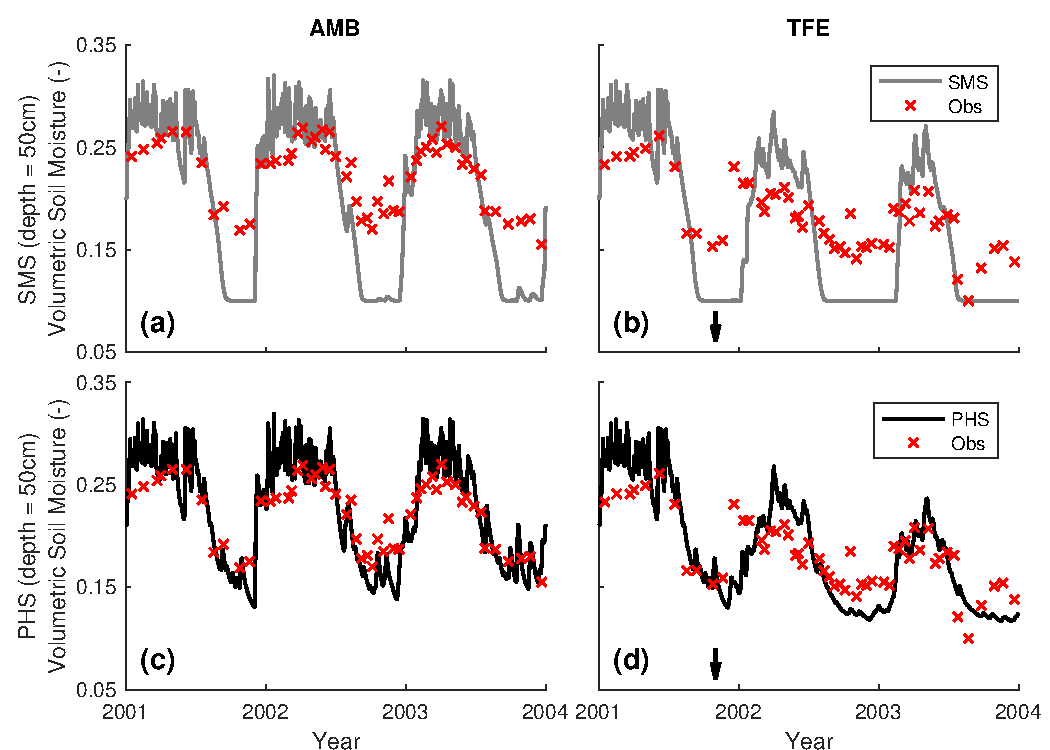
\includegraphics[width=30pc]{../figs3/sm2.pdf}
     \caption{Volumetric soil moisture (-) over time under ambient and TFE conditions at depth of 50cm.
     (a/b) SMS
     (c/d) PHS.
     RMSE are 0.048, 0.049, 0.022, and 0.029.
     Arrows indicate start of TFE. Figure \ref{supp:sm2} shows the same plots at 7 other soil depths. }
     \label{fig:sm2}
  \end{figure}

              \begin{figure}[h]
     \centering
     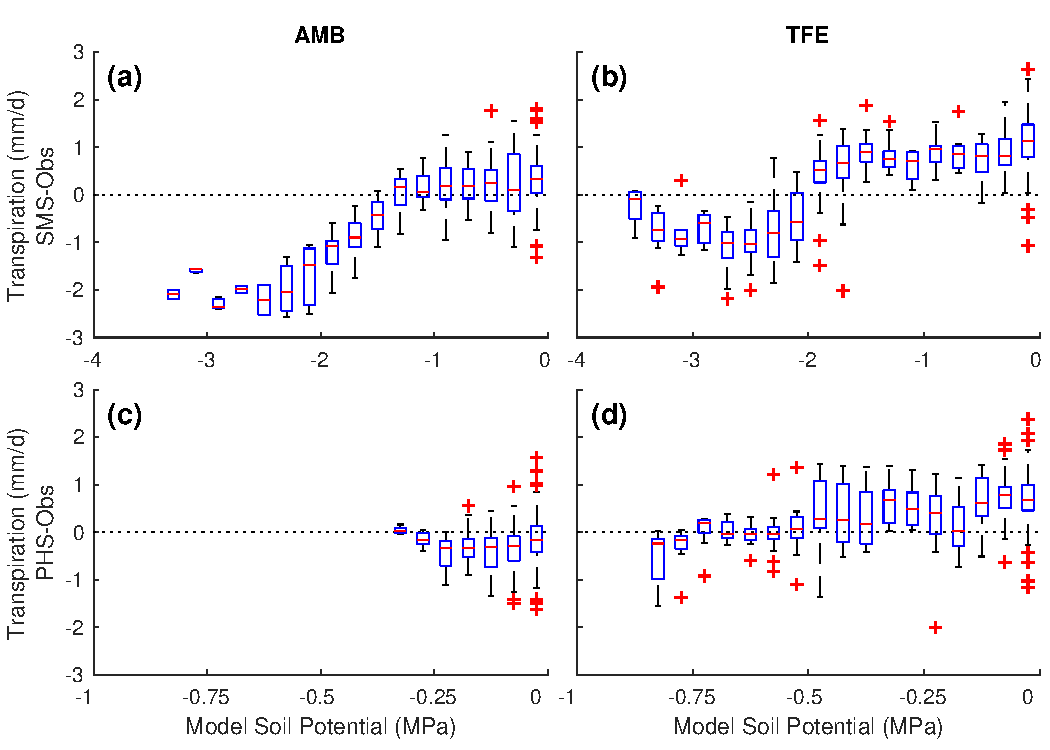
\includegraphics[width=30pc]{../figs3/sm3.pdf}
     \caption{Binned boxplot showing the difference between modeled and observed transpiration (mm/d) versus model soil potential.
     Red lines are drawn at the median, with boxes spanning the interquartile range.
     The two models use different root water uptake paradigms, from which we define different operators for column effective soil potential.
     For SMS we average over the soil column weighted by root fraction and over time (daily mean).
     For PHS we use predawn (5h) root water potential.
     Bin widths are 0.2 MPa for SMS (a,b) and 0.05 MPa for PHS (c,d).
}
     \label{fig:cool}
  \end{figure}
          \clearpage

\clearpage

\appendix
%====================
%  APPENDIX
%====================

\section{Supplementary Figures}


      \begin{figure}[h]
     \centering
     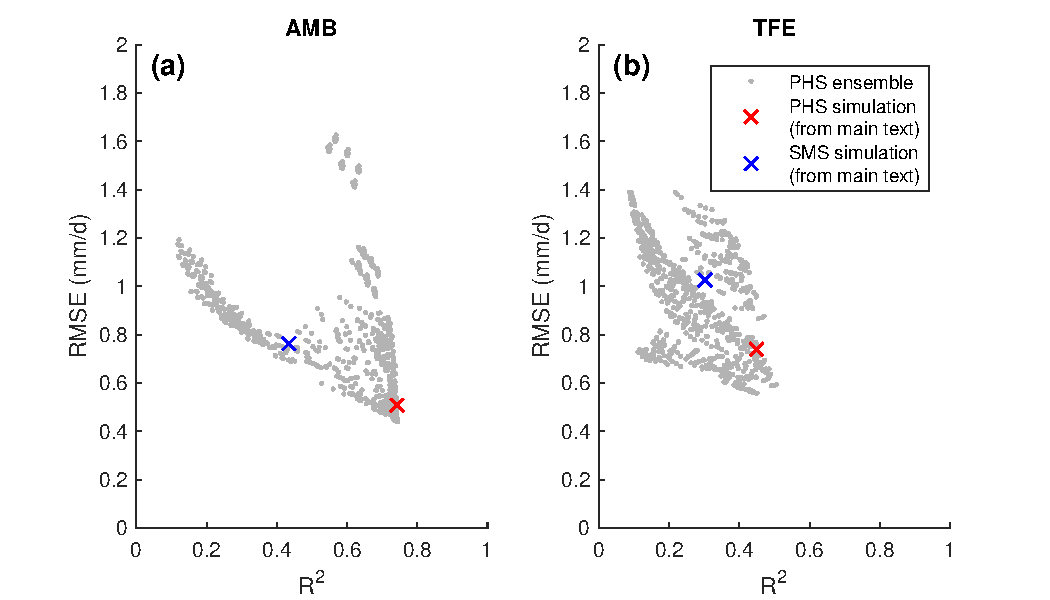
\includegraphics[width=30pc]{../figs3/ens.pdf}
     \caption{Parameter tuning exercise.
     }
     \label{supp:ens}
       \end{figure}
         \clearpage

      \begin{figure}[h]
     \centering
     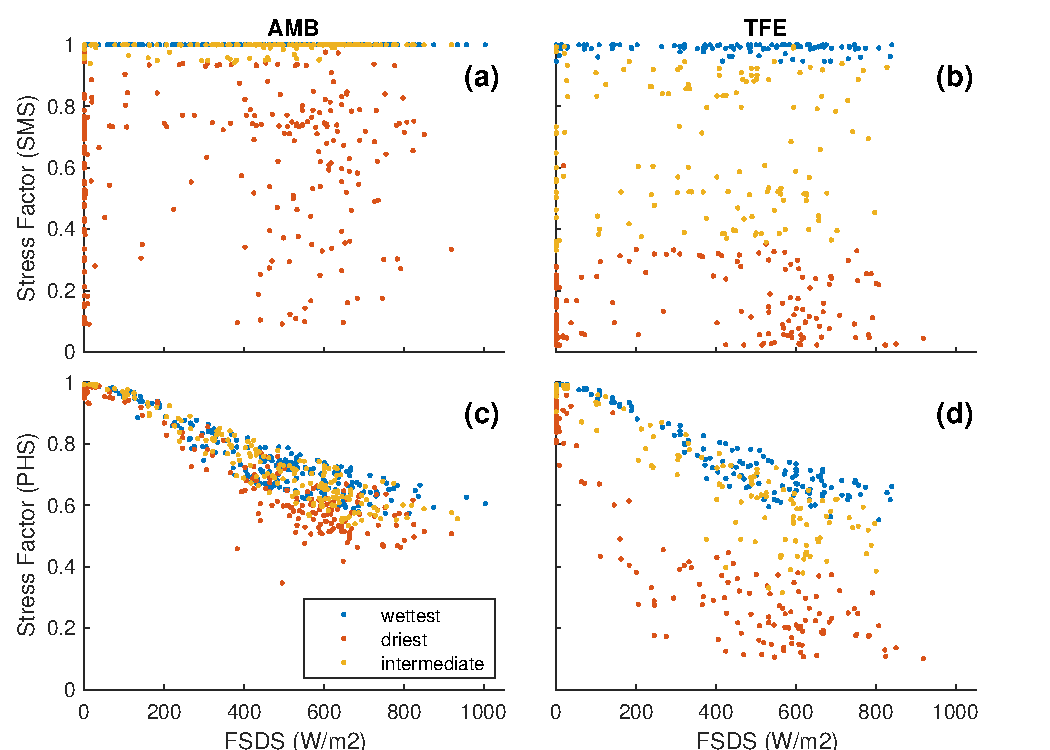
\includegraphics[width=30pc]{../figs3/suppstress.pdf}
     \caption{Water stress factor versus downwelling shortwave radiation (2002-2003), for timesteps with VPD between 1 and 1.0559 kPa (n=470).
     VPD is controlled to highlight the relationship with downwelling radiation, the reverse (controlling for radiation) is shown in Figure \ref{fig:stress2}.
     For SMS (a,b), data are subdivided based on average soil matric potential, weighted by root fraction.
     For PHS (c,d), data are subdivided based on predawn (5h) root water potential.
     Blue dots represent the wettest tercile, yellow dots represent the intermediate tercile, and red dots represent the driest tercile.
     }
     \label{supp:fsds}
       \end{figure}
         \clearpage

 

        \begin{figure}[h]
     \centering
     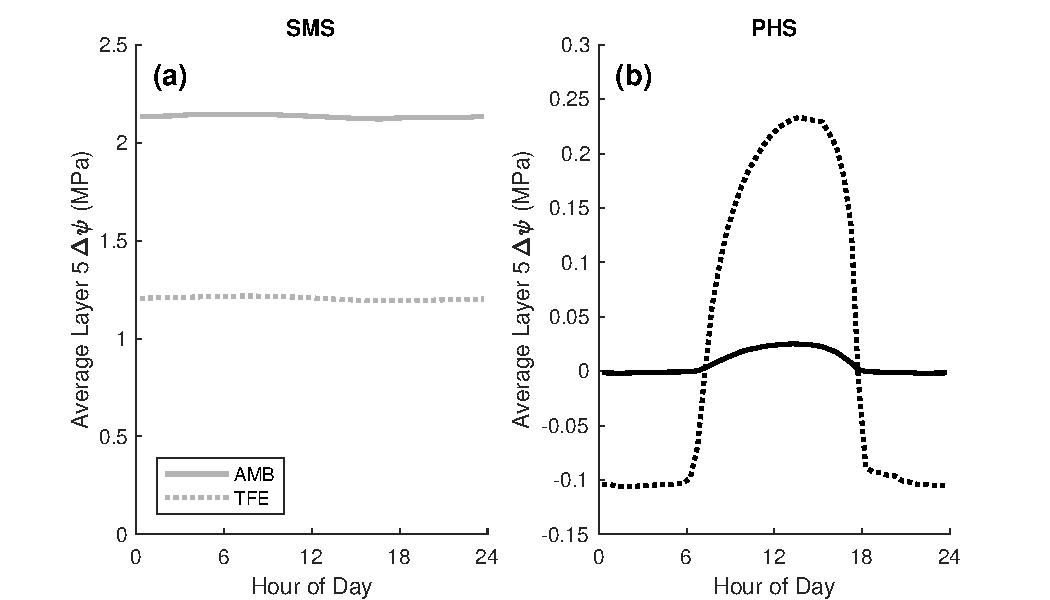
\includegraphics[width=30pc]{../figs3/suppdp.pdf}
     \caption{To complement Figure 6}
     \label{supp:cond}
  \end{figure}
  \clearpage
  
  
  \begin{figure}[h]
     \centering
     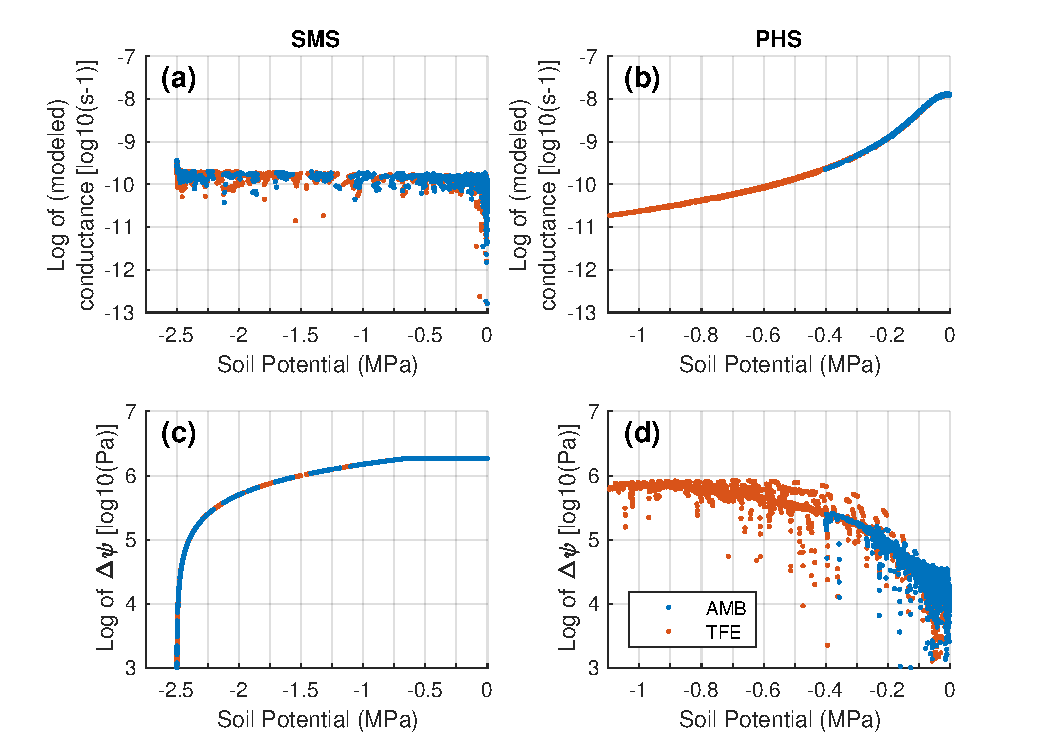
\includegraphics[width=30pc]{../figs3/suppcond.pdf}
     \caption{Log of conductance versus soil potential for Soil Layer 3 (2003).
     Only midday (12h-14h) timesteps are shown to emphasize relationship with soil potential.}
     \label{supp:cond2}
  \end{figure}
  \clearpage


  
      \begin{figure}[h]
     \centering
     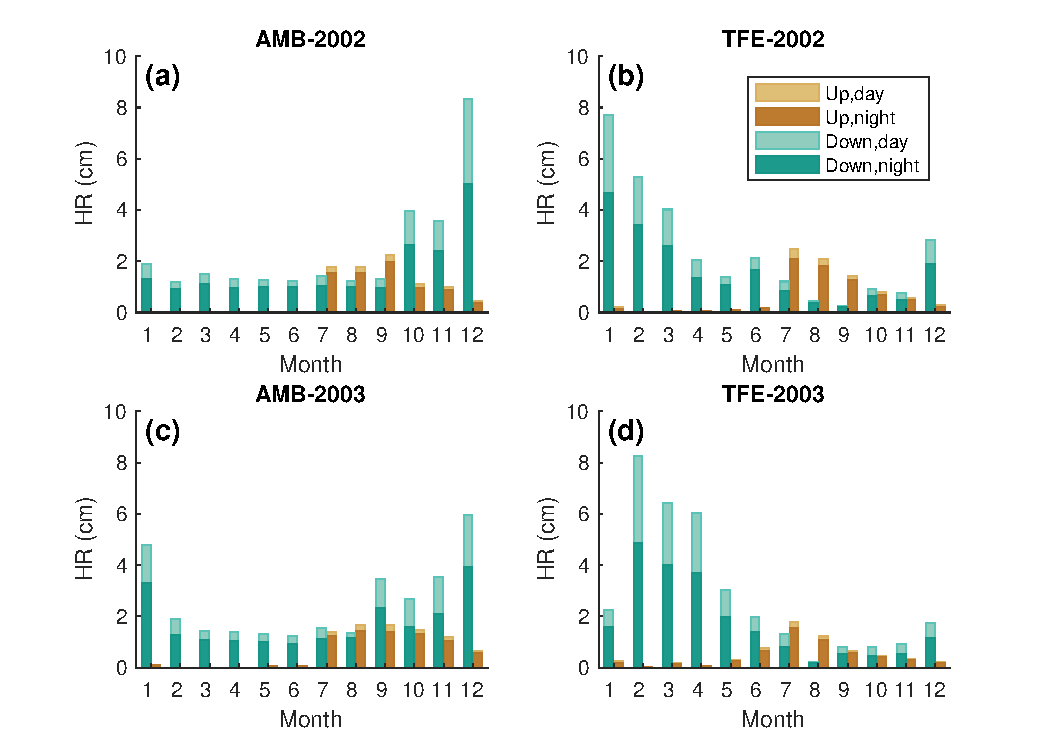
\includegraphics[width=30pc]{../figs3/hr2}
     \caption{PHS hydraulic distribution during 2003. Alternative version partitioning by direction.}
     \label{supp:hr}
  \end{figure}
  \clearpage
  



  
  
        \clearpage
    \begin{figure}[h]
     \centering
     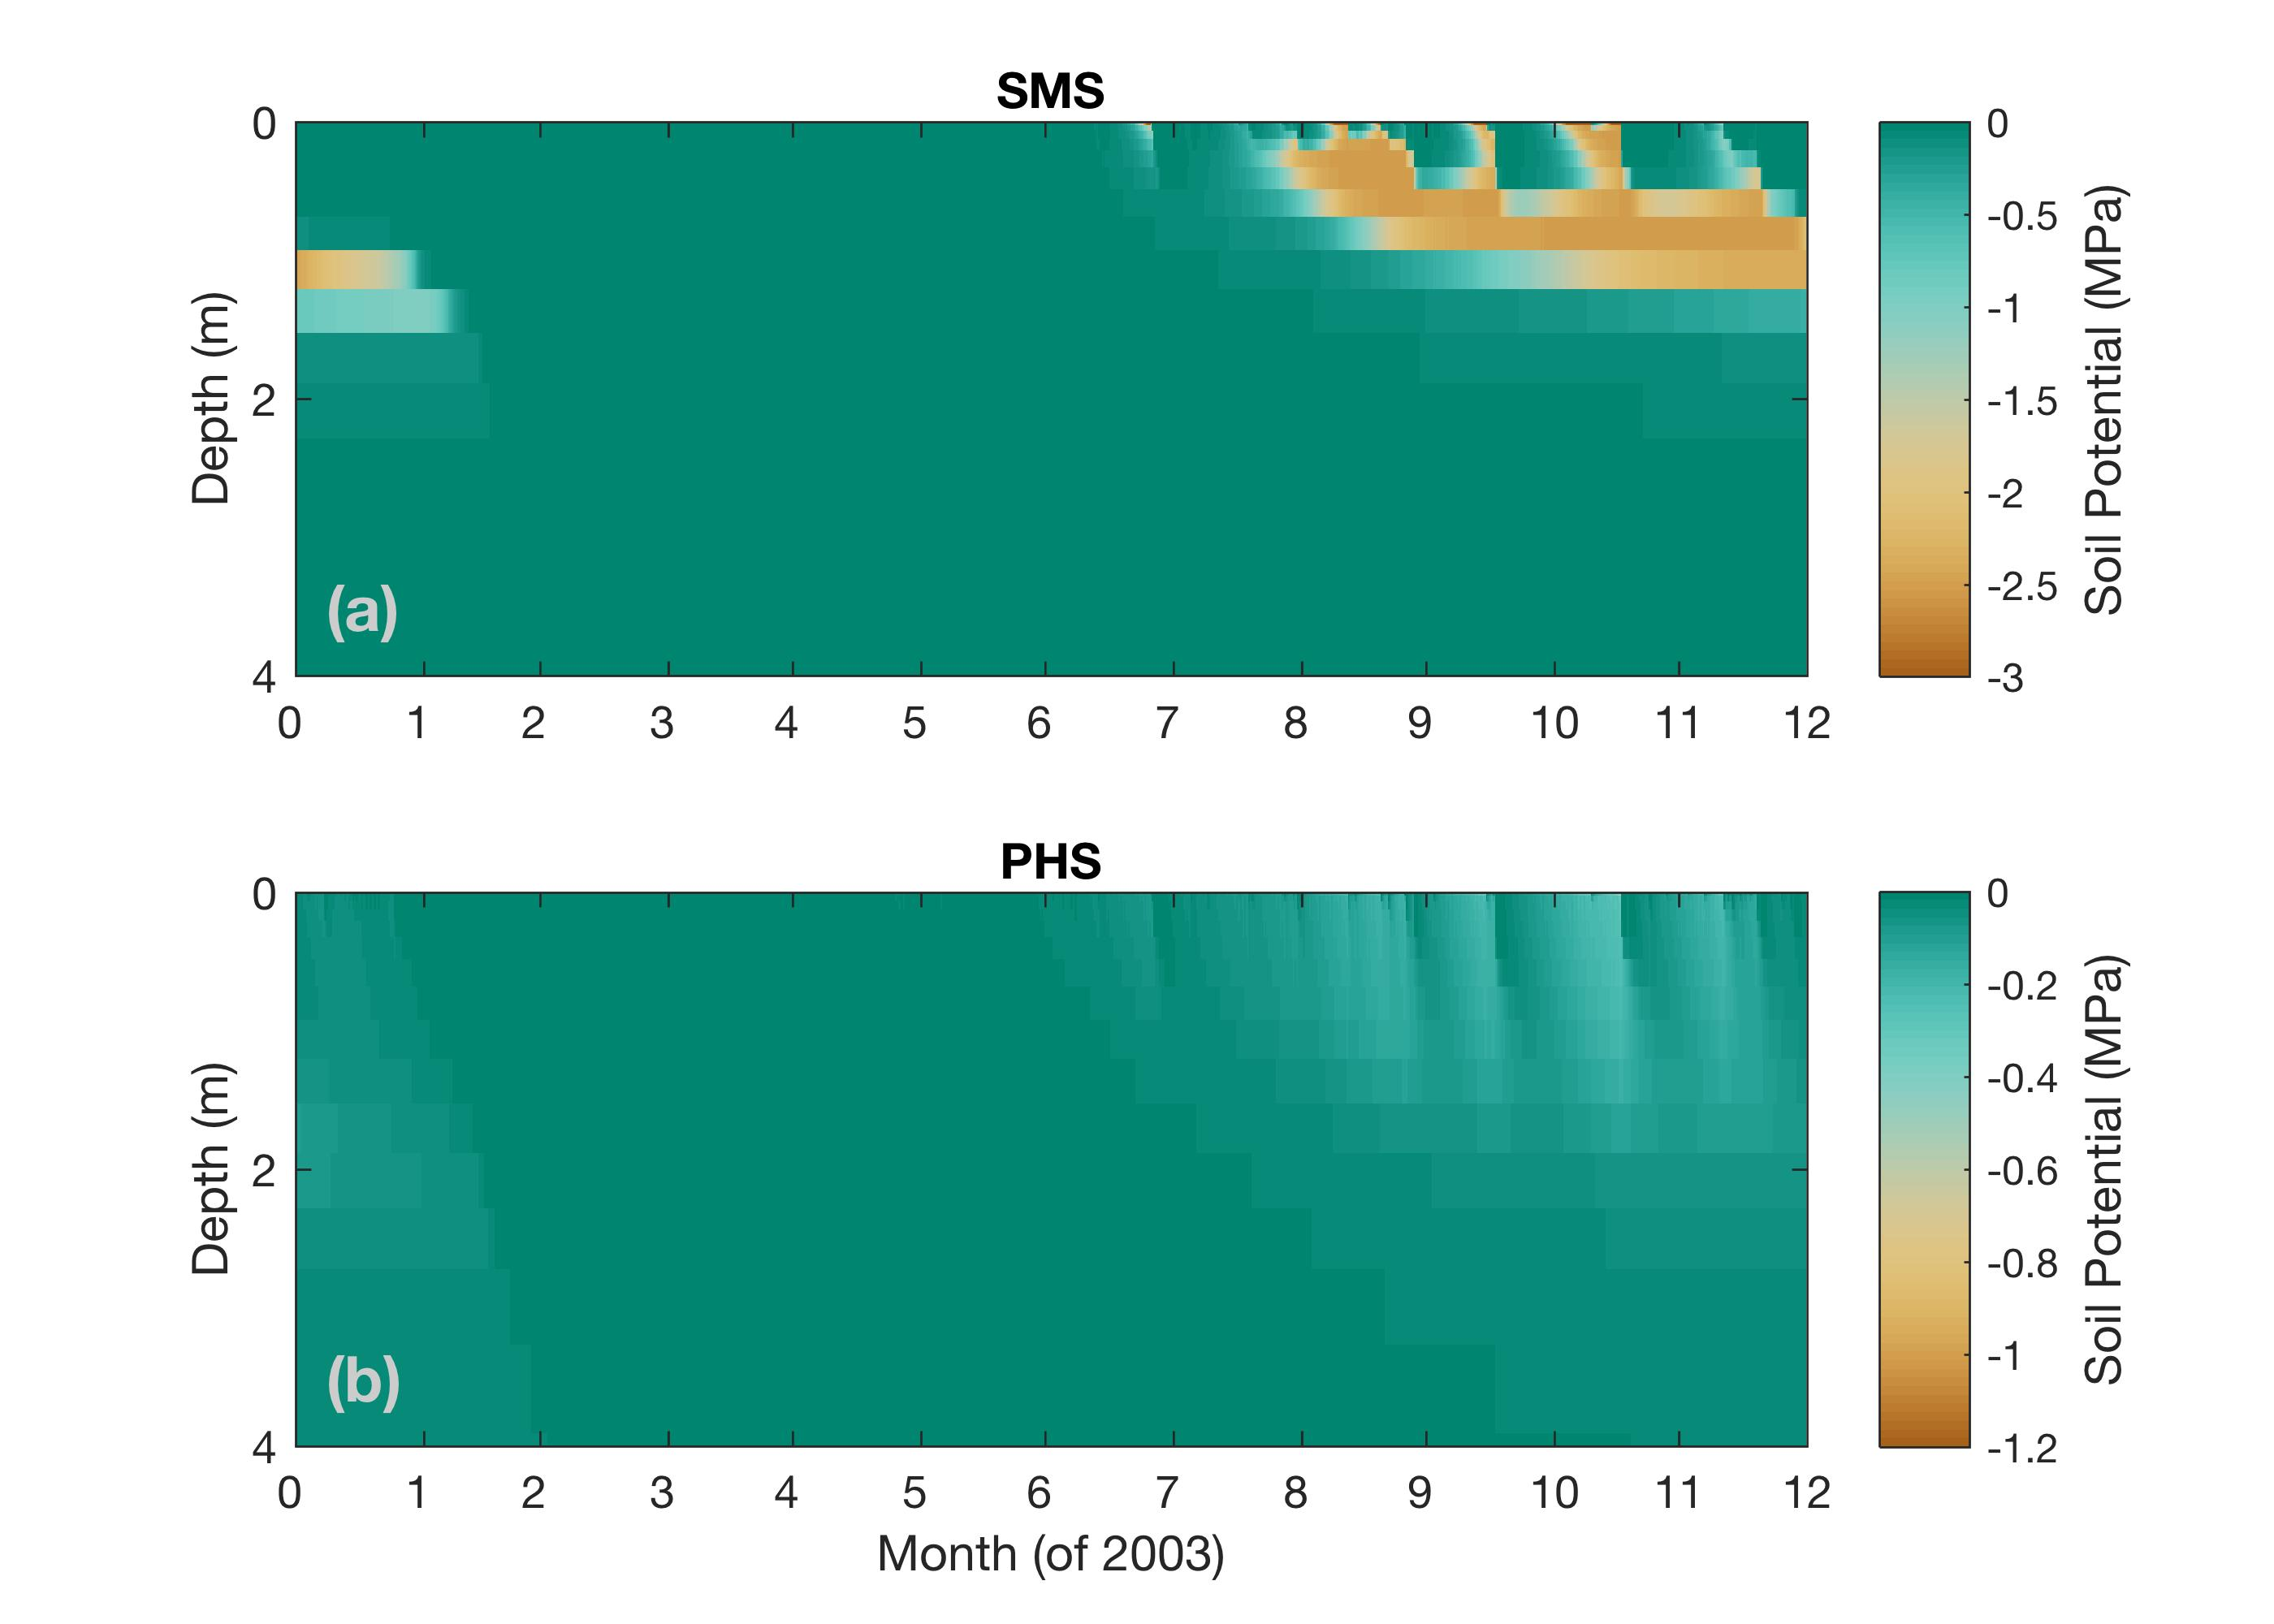
\includegraphics[width=30pc]{../figs3/suppsmp.jpg}
     \caption{Vertical profile of soil water potential (MPa) through time under ambient through-fall conditions, for
     (a) PHS, and 
     (b) SMS.
     Note that color axes are different. }
     \label{supp:sm}
  \end{figure}
  

    \begin{figure}[h]
     \centering
     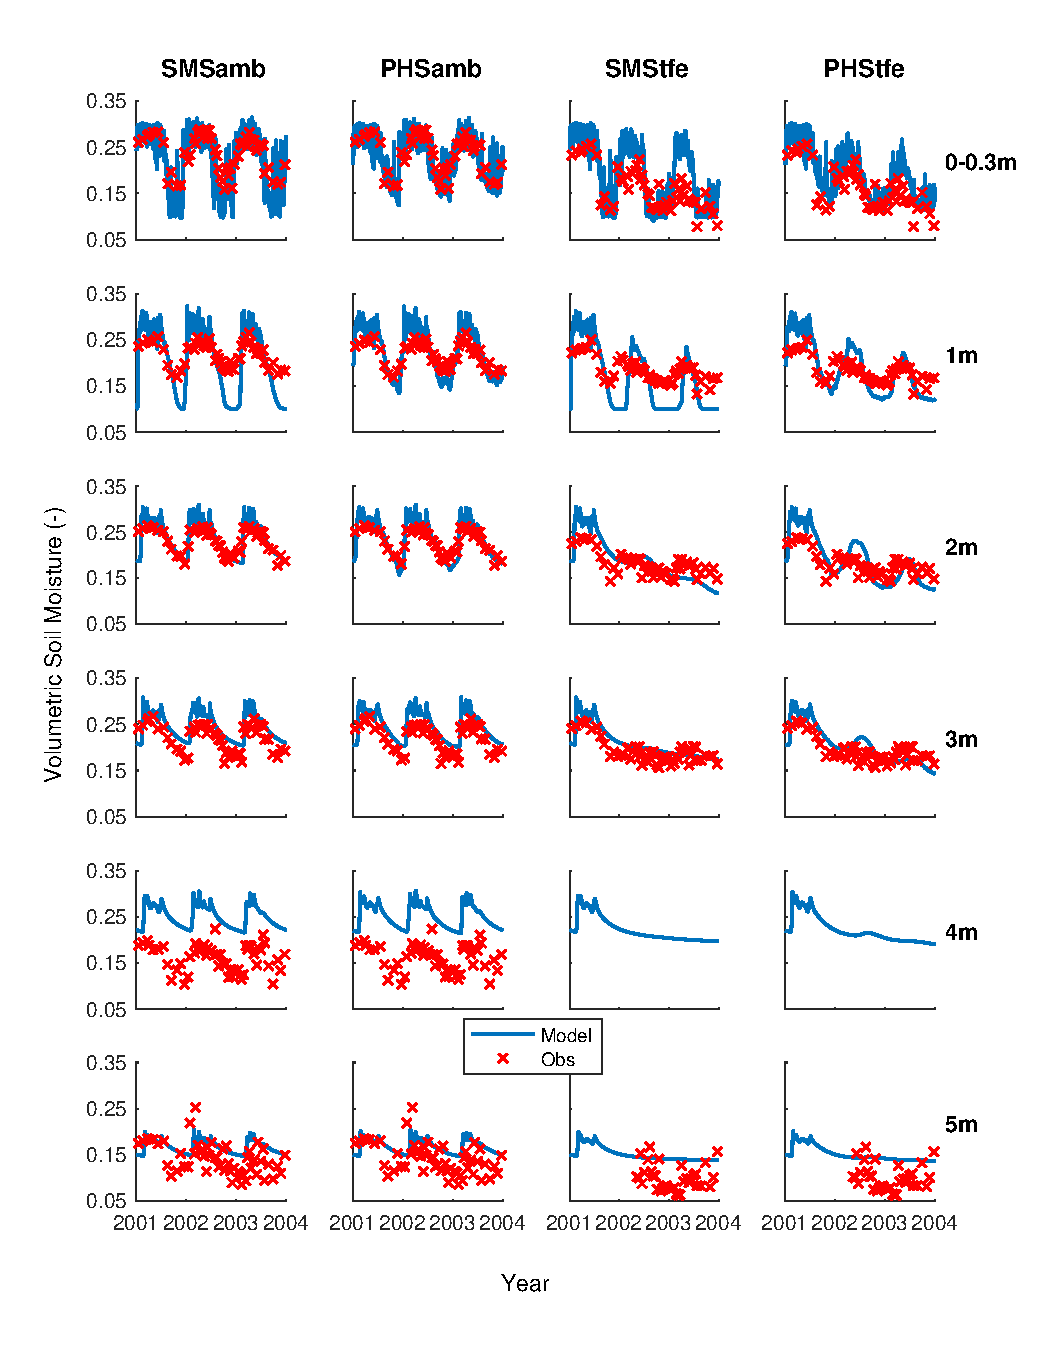
\includegraphics[width=30pc]{../figs3/suppsm2.pdf}
     \caption{Time series of soil moisture by soil layer.
     Complements Figure \ref{fig:sm}}
     \label{supp:sm2}
  \end{figure}
          \clearpage
          
     \begin{figure}[h]
     \centering
     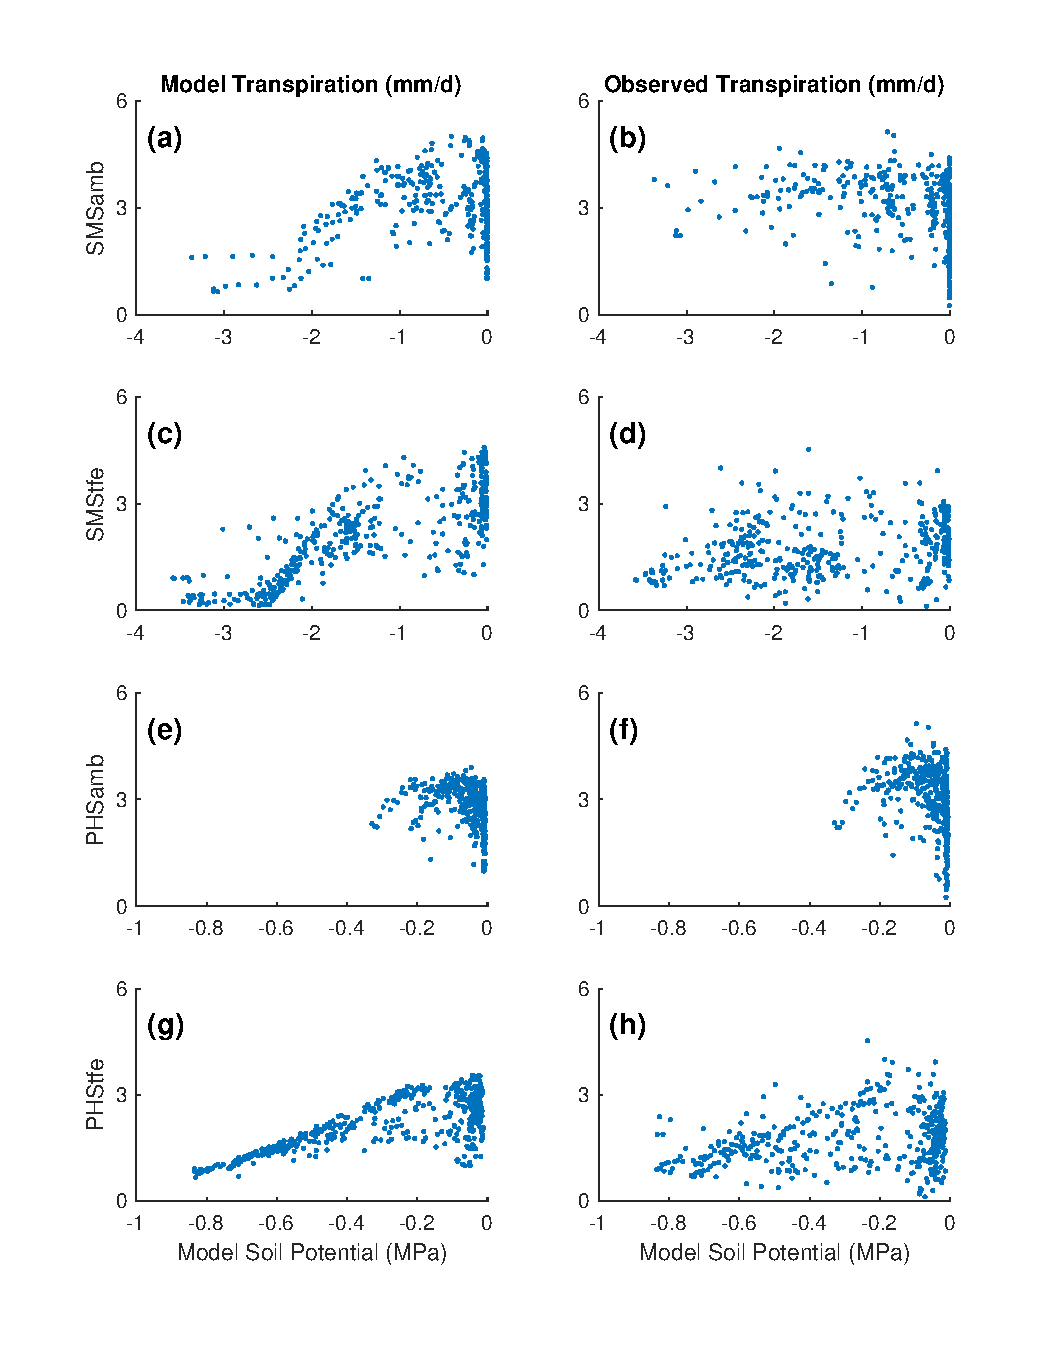
\includegraphics[width=30pc]{../figs3/suppcool.pdf}
     \caption{Modeled (left column) and observed (right column) transpiration  vs. model soil potential.
     Complements Figure \ref{fig:cool}}
     \label{supp:cool}
  \end{figure}
          \clearpage
          



\section{Appendix to Model Description}

% Details on water supply
\subsection{Details of Water Supply}

PHS resolves flow across four different segments, soil-to-root, root-to-stem, stem-to-leaf, and leaf-to-transpiration.

Stem-to-leaf. The area bases are sunlit and shaded leaf area, respectively. 
Note that gravity is assumed negligible here. 
Likewise there is no length scaling applied to maximum conductance. 
Therefore the input parameters for $k_{1,\text{max}}$ should be conductances ($s^{-1}$).

\begin{linenomath*} \begin{equation} \begin{aligned}
q_{1a} &= k_{1} \cdot \text{LAI-sun}  \cdot \left( \psi_{\text{stem}}-\psi_{\text{sun-leaf}}\right) \\
q_{1b} &= k_{1} \cdot \text{LAI-shade} \cdot  \left( \psi_{\text{stem}}-\psi_{\text{shade-leaf}}\right)
\end{aligned} \end{equation} \end{linenomath*}

\begin{linenomath*} \begin{equation}
k_{1} = k_{1,\text{max}} \cdot f\left(\psi_{\text{stem}}\right)
\end{equation} \end{linenomath*}

\begin{linenomath*} \begin{equation} \begin{aligned}
f\left(\psi\right)=2^{-\left(\dfrac{\psi}{p_{50}}\right)^{c_k}}
\end{aligned} \end{equation} \end{linenomath*}

Root-to-stem. The area basis is stem area index. 
The parameter is maximum stem xylem conductivity ($K_{2,\text{max}}$).
Stem conductance ($k_2$) is the result of scaling maximum conductivity by the tree height ($h$)
and applying loss relative to maximum conductance via the vulnerability curve $f\left(\psi_{\text{root}}\right)$. 
\begin{linenomath*} \begin{equation}
q_2 = k_2 \cdot  \text{SAI}  \cdot \left( \psi_{\text{root}}-\psi_{\text{stem}}-\rho g h\right)
\end{equation} \end{linenomath*}
\begin{linenomath*} \begin{equation}
k_2 = \dfrac{K_{2,\text{max}}}{h} \cdot f\left(\psi_{\text{root}}\right)
\end{equation} \end{linenomath*}

Soil-to-root. Area basis is RAI in soil layer $i$, which is based on the layer root fraction times the
total root area. Total root area we have as the summed stem and leaf area indices multiplied by a relative
root area parameter ($f_{\text{root}}$).
The vertical root distribution is defined by the layer root fraction ($r_i$), which follows a one-parameter 
(by PFT) power law decay following \citet{jackson1996}.

\begin{linenomath*} \begin{equation}
q_{3,i} = k_{3,i} \cdot  \text{RAI}_i  \cdot \left( \psi_{\text{soil,i}}-\psi_{\text{root}}-\rho g z_i\right)
\end{equation} \end{linenomath*}
\begin{linenomath*} \begin{equation}
\text{RAI}_i=f_{\text{root}} \cdot \left( \text{SAI} + \text{LAI} \right) \cdot r_i
\label{eq:rai}
\end{equation} \end{linenomath*}
\begin{linenomath*} \begin{equation}
k_{3,i} = \dfrac{k_{r,i}+k_{s,i}}{k_{r,i}\cdot k_{s,i}}
\end{equation} \end{linenomath*}
\begin{linenomath*} \begin{equation}
k_{r,i} = \dfrac{K_{r,\text{max}}}{l_i} f \left(\psi_{\text{soil,i}}\right)
\end{equation} \end{linenomath*}
\begin{linenomath*} \begin{equation}
l_i = z_i + x
\end{equation} \end{linenomath*}
\begin{linenomath*} \begin{equation}
k_{s,i} = \dfrac{K_{s,i}}{d}
\end{equation} \end{linenomath*}

The conductance $k_{3,i}$ reflects two resistors in series, from soil-to-root ($k_{s,i}$) and through the
root tissue ($k_{r,i}$).
The root tissue conductance is attenuated via the vulnerability curve framework. 
The input parameter is maximum root xylem conductivity, on the basis of RAI as defined above.
The root conductivity is scaled by the conducting length, which is estimated as the sum of soil layer depth ($z_i$)
and average lateral extent ($x$, static parameter).
The soil conductivity $K_{s,i}$ is calculated from the layer soil matric potential ($\psi_s$) 
and soil properties following \citet{clapp1978} as described in \citet{oleson2013}.
The soil conductance ($k_{s,i}$) is the result of scaling the conductivity by $d$, 
 the distance between roots estimated following \citet{williams1996} and \citet{bonan2014}

The challenge here is obviously getting your head around all the parameters.

% Details on water demand
\subsection{Details of Water Demand}

% Details on phs solution
\subsection{Details of Solution}


The continuity of water flow through the system yields four equations
   \begin{linenomath*} \begin{equation}
   \begin{aligned}
   E_{sun}&=q_{1a}\\
   E_{shade}&=q_{1b}\\
   q_{1a}+q_{1b}&=q_2\\
   q_2&=\sum_{i=1}^{nlevsoi}{q_{3,i}}
   \end{aligned}
   \end{equation} \end{linenomath*}

We seek the set of vegetation water potential values (four unknowns), 

   \begin{linenomath*} \begin{equation}
   \psi=\left[ \begin {array}{c} 
   \psi_{sunleaf}\cr\psi_{shadeleaf}\cr\psi_{stem}\cr\psi_{root}
   \end {array} \right] 
   \end{equation} \end{linenomath*}

that satisfies these equations, as forced by the soil moisture and atmospheric state. 

Each flux on the schematic can be represented in terms of the relevant water potentials. 

Defining the transpiration fluxes:


   \begin{linenomath*} \begin{equation}
   \begin{aligned}
   E_{sun} &= E_{sun,max} \cdot 2^{-\left(\dfrac{\psi_{sunleaf}}{p50_e}\right)^{c_k}} \\
   E_{shade} &= E_{shade,max} \cdot 2^{-\left(\dfrac{\psi_{shadeleaf}}{p50_e}\right)^{c_k}} 
   \end{aligned}
   \end{equation} \end{linenomath*}

Defining the water supply fluxes:

   \begin{linenomath*} \begin{equation}
   \begin{aligned}
   q_{1a}&=k_{1a,max}\cdot 2^{-\left(\dfrac{\psi_{stem}}{p50_1}\right)^{c_k}} \cdot\mbox{LAI}_{sun}\cdot\left(\psi_{stem}-\psi_{sunleaf} \right) \\
   q_{1b}&=k_{1b,max}\cdot 2^{-\left(\dfrac{\psi_{stem}}{p50_1}\right)^{c_k}}\cdot\mbox{LAI}_{shade}\cdot\left(\psi_{stem}-\psi_{shadeleaf} \right) \\
   q_2&=\dfrac{k_{2,max}}{z_2} \cdot 2^{-\left(\dfrac{\psi_{root}}{p50_2}\right)^{c_k}} \cdot SAI \cdot \left( \psi_{root} - \psi_{stem} - \Delta \psi_z  \right) \\
   q_{soil}&=\sum_{i=1}^{nlevsoi}{q_{3,i}}=\sum_{i=1}^{nlevsoi}{k_{3,i}\cdot RAI\cdot\left(\psi_{soil,i}-\psi_{root} + \Delta\psi_{z,i} \right)}
   \end{aligned}
   \end{equation} \end{linenomath*}

We're looking to find the vector $\psi$
that fits with soil and atmospheric forcings while satisfying water flow continuity. 
Due to the model non-linearity, we use a linearized explicit approach, iterating with Newton's method. 
The initial guess is the solution for $\psi$ (vector) from the previous time step. 
The general framework, from iteration $m$ to $m+1$ is:

   \begin{linenomath*} \begin{equation} 
   \begin{aligned}
   q^{m+1}&=q^m+\dfrac{\delta q}{\delta\psi}\Delta\psi \\
   \psi^{m+1}&=\psi^{m}+\Delta\psi
   \end{aligned}
   \end{equation} \end{linenomath*}

So for our first flux balance equation, at iteration $m+1$, we have:

   \begin{linenomath*} \begin{equation} 
   E_{sun}^{m+1}=q_{1a}^{m+1}
   \end{equation} \end{linenomath*}

Which can be linearized to:

   \begin{linenomath*} \begin{equation} 
   E_{sun}^{m}+\dfrac{\delta E_{sun}}{\delta\psi}\Delta\psi=q_{1a}^{m}+\dfrac{\delta q_{1a}}{\delta\psi}\Delta\psi
   \end{equation} \end{linenomath*}

And rearranged to be:

   \begin{linenomath*} \begin{equation} 
   \dfrac{\delta q_{1a}}{\delta\psi}\Delta\psi-\dfrac{\delta E_{sun}}{\delta\psi}\Delta\psi=E_{sun}^{m}-q_{1a}^{m}
   \end{equation} \end{linenomath*}

And for the other 3 flux balance equations:

   \begin{linenomath*} \begin{equation} 
   \begin{aligned}
   \dfrac{\delta q_{1b}}{\delta\psi}\Delta\psi-\dfrac{\delta E_{sha}}{\delta\psi}\Delta\psi&=E_{sha}^{m}-q_{1b}^{m} \\
   \dfrac{\delta q_2}{\delta\psi}\Delta\psi-\dfrac{\delta q_{1a}}{\delta\psi}\Delta\psi-\dfrac{\delta q_{1b}}{\delta\psi}\Delta\psi&=q_{1a}^{m}+q_{1b}^{m}-q_2^{m} \\
   \dfrac{\delta q_{soil}}{\delta\psi}\Delta\psi-\dfrac{\delta q_2}{\delta\psi}\Delta\psi&=q_2^{m}-q_{soil}^{m}
   \end{aligned}
   \end{equation} \end{linenomath*}

Putting all four together in matrix form:

   \begin{linenomath*} \begin{equation} 
   \left[ \begin {array}{c}
   \dfrac{\delta q_{1a}}{\delta\psi}-\dfrac{\delta E_{sun}}{\delta\psi} \cr
   \dfrac{\delta q_{1b}}{\delta\psi}-\dfrac{\delta E_{sha}}{\delta\psi} \cr
   \dfrac{\delta q_2}{\delta\psi}-\dfrac{\delta q_{1a}}{\delta\psi}-\dfrac{\delta q_{1b}}{\delta\psi} \cr
   \dfrac{\delta q_{soil}}{\delta\psi}-\dfrac{\delta q_2}{\delta\psi}
   \end {array} \right]
   \Delta\psi=
   \left[ \begin {array}{c}
   E_{sun}^{m}-q_{1a}^{m} \cr
   E_{sha}^{m}-q_{1b}^{m} \cr
   q_{1a}^{m}+q_{1b}^{m}-q_2^{m} \cr
   q_2^{m}-q_{soil}^{m}
   \end {array} \right]
   \end{equation} \end{linenomath*}

Now to expand the left-hand side, from vector $\psi$ to the four distinct plant water potential nodes, noting that many derivatives are zero (e.g. $\dfrac{\delta E_{sun}}{\delta\psi_{sha}}=0$)

Introducing the notation:
$A\Delta\psi=b$

   \begin{linenomath*} \begin{equation} 
   \Delta\psi=\left[ \begin {array}{c}
   \Delta\psi_{sunleaf} \cr
   \Delta\psi_{shadeleaf} \cr
   \Delta\psi_{stem} \cr
   \Delta\psi_{root}
   \end {array} \right] 
   \end{equation} \end{linenomath*}

   \begin{linenomath*} \begin{equation} 
   A=
   \left[ \begin {array}{cccc}
   \dfrac{\delta q_{1a}}{\delta \psi_{sun}}-\dfrac{\delta E_{sun}}{\delta \psi_{sun}}&0&\dfrac{\delta q_{1a}}{\delta \psi_{stem}}&0\cr
   0&\dfrac{\delta q_{1b}}{\delta \psi_{sha}}-\dfrac{\delta E_{sha}}{\delta \psi_{sha}}&\dfrac{\delta q_{1b}}{\delta \psi_{stem}}&0\cr
   -\dfrac{\delta q_{1a}}{\delta \psi_{sun}}&
   -\dfrac{\delta q_{1b}}{\delta \psi_{sha}}&
   \dfrac{\delta q_2}{\delta \psi_{stem}}-\dfrac{\delta q_{1a}}{\delta \psi_{stem}}-\dfrac{\delta q_{1b}}{\delta \psi_{stem}}&
   \dfrac{\delta q_2}{\delta \psi_{root}}\cr
   0&0&-\dfrac{\delta q_2}{\delta \psi_{stem}}&\dfrac{\delta q_{soil}}{\delta \psi_{root}}-\dfrac{\delta q_2}{\delta \psi_{root}}
   \end {array} \right]
   \end{equation} \end{linenomath*}

   \begin{linenomath*} \begin{equation} 
   b=
   \left[ \begin {array}{c}
   E_{sun}^{m}-q_{b1}^{m} \cr
   E_{sha}^{m}-q_{b2}^{m} \cr
   q_{b1}^{m}+q_{b2}^{m}-q_{stem}^{m} \cr
   q_{stem}^{m}-q_{soil}^{m}
   \end {array} \right]
   \end{equation} \end{linenomath*}

Now we compute all the entries for $A$ and $b$ based on the soil moisture and maximum transpiration forcings and can solve to find:

   \begin{linenomath*} \begin{equation} 
   \Delta\psi=A^{-1}b
   \end{equation} \end{linenomath*}

   \begin{linenomath*} \begin{equation} 
   \psi_{m+1}=\psi_m+\Delta\psi
   \end{equation} \end{linenomath*}

We iterate until $b\to 0$, signifying water flux balance through the system. The result is a final set of water potentials ( $\psi_{root}$, $\psi_{xylem}$, $\psi_{shadeleaf}$, $\psi_{sunleaf}$) satisfying non-divergent water flux through the system. 
The magnitude of the water flux is driven by soil matric potential and unstressed ( $\beta_t=1$) transpiration. 

We use the transpiration solution (corresponding to the final solution for $\psi$) to compute stomatal conductance. The stomatal conductance is then used to compute $\beta_t$. 

   \begin{linenomath*} \begin{equation} 
   \beta_{t,sun} = \dfrac{g_{s,sun}}{g_{s,sun,\beta_t=1}} 
   \end{equation} \end{linenomath*}

   \begin{linenomath*} \begin{equation} 
   \beta_{t,shade} = \dfrac{g_{s,shade}}{g_{s,shade,\beta_t=1}} 
   \end{equation} \end{linenomath*}

The $\beta_t$ values are used in the Photosynthesis module (see section \ref{sect:A}) to apply water stress. 
The solution for $\psi$ is saved as a new variable (vegetation water potential) and is indicative of plant water status.
The soil-to-root fluxes $\left( q_{3,1},q_{3,2},\text{...},q_{3,n}\right)$ are used as the soil transpiration sink in the Richards' equation subsurface flow equations.

    Furthermore several simplifications were made that decrease the numerical complexity.
    For the purposes of the PHS solution, soil potentials are assumed constant during each timestep.
    Plant tissue water storage (capacitance) is not represented, whereby the solution does not
    depend on the previous timestep and has no time derivatives.

\acknowledgments
 = enter acknowledgments here =

PIerre: Text I removed
While there are disagreements about soil moisture trends globally \citep{dai2013,sheffield2012}, 
Amazonia has experienced and a lengthening dry season \citep{fu2013} and faces projections of increasing frequency of extreme El Ni\~no events \citep{cai2014}

%====================
%   REFERENCES
%====================
\nocite{*} 
\bibliography{refs/all}


\listofchanges


\end{document}


